% lecture2_ro.tex -- GENERATED by build_L2.py from L2_numbers.json; do not edit by hand.
\documentclass[10pt,aspectratio=169,t]{beamer}
% =============================================================================
% nn_preamble.tex -- shared Beamer preamble of Neural Networks and Deep Learning (NN)
% Used by every lecture: lectures/Lk/lecturek.tex does
%   \documentclass[10pt,aspectratio=169,t]{beamer}
%   % =============================================================================
% nn_preamble.tex -- shared Beamer preamble of Neural Networks and Deep Learning (NN)
% Used by every lecture: lectures/Lk/lecturek.tex does
%   \documentclass[10pt,aspectratio=169,t]{beamer}
%   % =============================================================================
% nn_preamble.tex -- shared Beamer preamble of Neural Networks and Deep Learning (NN)
% Used by every lecture: lectures/Lk/lecturek.tex does
%   \documentclass[10pt,aspectratio=169,t]{beamer}
%   \input{../common/nn_preamble}
%   \nnlecture{k}{Lecture title}
% Logos live in lectures/common/logos/, charts in lectures/Lk/charts/.
% Do NOT add \hfuzz / \vfuzz / \hbadness here: overfull boxes must be fixed, not hidden.
% =============================================================================

\usetheme{default}
\setbeamersize{text margin left=7mm, text margin right=7mm}

% ---------------------------------------------------------------- packages
\usepackage[utf8]{inputenc}
\usepackage[T1]{fontenc}
\usepackage{lmodern}
\usepackage{amsmath, amssymb}
\usepackage{mathtools}
\usepackage{bm}
\usepackage{tikz}
\usetikzlibrary{arrows.meta, positioning, calc, shapes.misc}
\usepackage{booktabs}
\usepackage{array}
\usepackage{graphicx}
\usepackage{colortbl}
\usepackage{xcolor}
\usepackage{multicol}
\hypersetup{colorlinks=true, linkcolor=MainBlue, urlcolor=MainBlue, citecolor=MainBlue}
\graphicspath{{../common/logos/}}   % charts are included with their language folder: charts/en/, charts/ro/

% ---------------------------------------------------------------- colours
\definecolor{MainBlue}{RGB}{26, 58, 110}
\definecolor{IDAred}{RGB}{205, 0, 0}
\definecolor{DarkGray}{RGB}{51, 51, 51}
\definecolor{FooterGray}{RGB}{100, 100, 100}
\definecolor{BlockGray}{RGB}{236, 238, 242}
\definecolor{KeynoteGray}{RGB}{218, 218, 218}
\definecolor{Crimson}{RGB}{190, 40, 50}
\definecolor{Forest}{RGB}{30, 110, 50}
\definecolor{Bitter}{RGB}{214, 150, 20}
% chart palette (same hex values and order as lectures/common/nn_plot.py SERIES)
\definecolor{Ser1}{HTML}{2A78D6}
\definecolor{Ser2}{HTML}{EB6834}
\definecolor{Ser3}{HTML}{1BAF7A}
\definecolor{Ser4}{HTML}{EDA100}
\definecolor{Ser5}{HTML}{E87BA4}
\definecolor{Ser6}{HTML}{008300}
\definecolor{Ser7}{HTML}{6250D6}
\definecolor{Ser8}{HTML}{E34948}

\setbeamertemplate{background}{%
  \begin{tikzpicture}[remember picture, overlay]
    \shade[shading=axis, shading angle=315, top color=white, bottom color=KeynoteGray]
      (current page.south west) rectangle (current page.north east);
  \end{tikzpicture}}
\setbeamercolor{background canvas}{bg=}
\setbeamercolor{structure}{fg=MainBlue}
\setbeamercolor{normal text}{fg=DarkGray}
\setbeamercolor{title}{fg=IDAred}
\setbeamercolor{frametitle}{fg=IDAred, bg=}
\setbeamercolor{block title}{bg=MainBlue, fg=white}
\setbeamercolor{block body}{bg=BlockGray, fg=DarkGray}
\setbeamercolor{block title alerted}{bg=Crimson, fg=white}
\setbeamercolor{block body alerted}{bg=Crimson!7, fg=DarkGray}
\setbeamercolor{block title example}{bg=Forest, fg=white}
\setbeamercolor{block body example}{bg=Forest!7, fg=DarkGray}
\setbeamercolor{item}{fg=MainBlue}
\setbeamerfont{frametitle}{size=\large, series=\bfseries}
\setbeamerfont{block title}{size=\small, series=\bfseries}
\setbeamertemplate{blocks}[rounded][shadow=false]
\setbeamertemplate{itemize item}{\color{MainBlue}$\boxdot$}
\setbeamertemplate{itemize subitem}{\color{MainBlue}\scriptsize$\blacktriangleright$}
% compact two-level lists: level 1 = main point, level 2 = details (no text outside bullets)
\setbeamerfont{itemize/enumerate subbody}{size=\footnotesize}
\setlength{\leftmargini}{1.1em}
\setlength{\leftmarginii}{1.1em}
\setbeamertemplate{itemize/enumerate body begin}{\setlength{\topsep}{0pt}\setlength{\partopsep}{0pt}\setlength{\parskip}{0pt}}
\setbeamertemplate{itemize/enumerate subbody begin}{\setlength{\topsep}{0pt}\setlength{\partopsep}{0pt}\setlength{\itemsep}{0pt}\vspace{-0.4ex}}

\setbeamertemplate{enumerate item}{\color{MainBlue}\insertenumlabel.}
\setlength{\leftmargini}{1.3em}
\setlength{\leftmarginii}{1.2em}
\setbeamertemplate{navigation symbols}{}
\setbeamertemplate{section in toc}{\color{MainBlue}$\blacktriangleright$~\inserttocsection}
\setbeamertemplate{caption}{\raggedright\insertcaption\par}
% frame subtitle = precise citation line under the claim title (Weron style)
\setbeamerfont{framesubtitle}{size=\footnotesize}
\setbeamercolor{framesubtitle}{fg=FooterGray}
% outline that reappears at every section with the current section highlighted
\setbeamertemplate{section in toc shaded}[default][35]
\setbeamertemplate{subsection in toc shaded}[default][35]
\setbeamertemplate{subsection in toc}{\leavevmode\leftskip=2.2em\color{DarkGray}\small\inserttocsubsection\par}
\AtBeginSection[]{{\begin{frame}{\txtoutline}\vspace{2mm}\small
  \tableofcontents[currentsection,hideothersubsections]\end{frame}}}

% ---------------------------------------------------------------- head and foot
\setbeamertemplate{headline}{%
  \vskip10pt%
  \hbox to \paperwidth{\hskip0.5cm%
    {\small\color{FooterGray}\renewcommand{\hyperlink}[2]{##2}\insertsectionhead}%
    \hfill\textcolor{FooterGray}{\small\insertframenumber}\hskip0.5cm}%
  \vskip4pt{\color{FooterGray}\hrule height 0.4pt}}
% footer as in the other courses (MFM, SFM): course name on the left, small sparkline on the right
\setbeamertemplate{footline}{%
  {\color{FooterGray}\hrule height 0.4pt}\vskip4pt%
  \hbox to \paperwidth{\hskip0.5cm%
    \textcolor{FooterGray}{\small\txtcourse}%
    \hfill\raisebox{-0.1em}{\begin{tikzpicture}[x=0.08em, y=0.08em, line width=0.4pt]
      \draw[FooterGray] (0,3) -- (1,4) -- (2,3.5) -- (3,5) -- (4,4) -- (5,6) -- (6,5.5) -- (7,4) -- (8,5) -- (9,7) -- (10,6) -- (11,5) -- (12,6.5) -- (13,8) -- (14,7) -- (15,6) -- (16,7.5) -- (17,9) -- (18,8) -- (19,7) -- (20,8.5) -- (21,10) -- (22,9) -- (23,8) -- (24,9.5);
    \end{tikzpicture}}\hskip0.5cm}%
  \vskip6pt}

% ---------------------------------------------------------------- title page
\defbeamertemplate*{title page}{nn}[1][]{%
  \vspace{0.15cm}
  \begin{center}
    \href{https://www.ase.ro}{
\includegraphics[height=0.9cm]{ase_logo.png}}\hspace{0.3cm}%
    \href{https://ipe.ro/new}{
\includegraphics[height=0.9cm]{acad_logo.png}}\hspace{0.3cm}%
    \href{https://theida.net}{
\includegraphics[height=0.9cm]{ida_logo.png}}\hspace{0.3cm}%
    \href{https://blockchain-research-center.com}{
\includegraphics[height=0.9cm]{brc_logo.png}}\hspace{0.3cm}%
    \href{https://www.ai4efin.ase.ro}{
\includegraphics[height=0.9cm]{ai4efin_logo.png}}\hspace{0.3cm}%
    \href{https://www.digital-finance-msca.com}{
\includegraphics[height=0.9cm]{msca_logo.png}}%
  \end{center}
  \vspace{0.45cm}
  \begin{center}
    \begin{minipage}{0.1\textwidth}\centering
      \href{https://quantlet.com}{
\includegraphics[height=0.9cm]{ql_logo.png}}\end{minipage}%
    \begin{minipage}{0.78\textwidth}\centering
      {\Large\bfseries\usebeamercolor[fg]{title}\inserttitle}\par\vspace{0.25cm}
      {\large\usebeamercolor[fg]{title}\insertsubtitle}\end{minipage}%
    \begin{minipage}{0.1\textwidth}\centering
      \href{https://quantinar.com}{
\includegraphics[height=0.9cm]{qr_logo.png}}\end{minipage}
  \end{center}
  \vfill
  \hspace{0.4cm}{\bfseries\insertauthor}\par\vspace{0.12cm}
  \hspace{0.4cm}\begin{minipage}[t]{0.92\textwidth}\raggedright\footnotesize\insertinstitute\end{minipage}
  \par\vspace{0.4cm}}

% ---------------------------------------------------------------- lecture metadata
\newcommand{\nnshort}{}
\newcommand{\nnnb}{notebooks}
\newcommand{\nnrepo}{https://github.com/danpele/NEURAL_BIZ/tree/main}
% language-dependent labels (English default; \nnromanian switches to Romanian, call it before \nnlecture)
\newcommand{\txtcourse}{Neural Networks and Deep Learning}
\newcommand{\txtlecture}{Lecture}
\newcommand{\txtoutline}{Outline}
\newcommand{\txtintuition}{In one sentence:}
\newcommand{\txtjob}{In practice:}
\newcommand{\txttry}{Experiment yourself:}
\newcommand{\txtwhere}{where}
\newcommand{\txtsim}{SIMULATED DATA (teaching illustration)}
\newcommand{\txtnbsuffix}{}
\newcommand{\txtinstitute}{Bucharest University of Economic Studies (ASE), Department of Statistics and Econometrics\\
    Romanian Academy, Institute for Economic Forecasting (IPE)\\
    IDA Institute Digital Assets \textbullet\ AI4EFin \textbullet\ MSCA Digital Finance}
\newcommand{\nnromanian}{%
  \renewcommand{\txtcourse}{Rețele neuronale și deep learning}%
  \renewcommand{\txtlecture}{Cursul}%
  \renewcommand{\txtoutline}{Cuprins}%
  \renewcommand{\txtintuition}{Pe scurt:}%
  \renewcommand{\txtjob}{În practică:}%
  \renewcommand{\txttry}{Exercițiu practic:}%
  \renewcommand{\txtwhere}{unde}%
  \renewcommand{\txtsim}{DATE SIMULATE (doar pentru ilustrare)}%
  \renewcommand{\txtnbsuffix}{\string_ro}%
  \renewcommand{\txtinstitute}{Academia de Studii Economice din București (ASE), Departamentul de Statistică și Econometrie\\
    Academia Română, Institutul de Prognoză Economică (IPE)\\
    IDA Institute Digital Assets \textbullet\ AI4EFin \textbullet\ MSCA Digital Finance}}
\newcommand{\nnlecture}[2]{%
  \renewcommand{\nnshort}{\txtlecture\ #1}%
  \renewcommand{\nnnb}{notebooks/L#1\string_notebook\txtnbsuffix.ipynb}%
  \title[NN]{\txtcourse}%
  \subtitle{\txtlecture\ #1: #2}%
  \author{Prof.\ dr.\ Daniel Traian PELE}%
  \institute{\txtinstitute}%
  \date{}}

% ---------------------------------------------------------------- teaching blocks (one message per frame)
% \intuition{one plain sentence}  ->  formula with every symbol defined  ->  real-data example  ->  \manager{one line}
\newcommand{\intuition}[1]{\begin{itemize}\item {\color{MainBlue}\textbf{\txtintuition}}~#1\end{itemize}\vspace{0.6mm}}
\newcommand{\manager}[1]{\colorbox{Forest!10}{\parbox{\dimexpr\linewidth-2\fboxsep\relax}{\footnotesize
  \begin{itemize}\setlength{\itemsep}{0pt}\item \textbf{\color{Forest}\txtjob}~#1\end{itemize}}}}
% Experiment yourself: pointer to the matching notebook section
\newcommand{\tryit}[1]{{\scriptsize\href{\nnrepo/\nnnb}{%
  \raisebox{-0.15em}{
\includegraphics[height=0.85em]{ql_logo.png}}\,\textbf{\txttry}~\color{MainBlue}#1}}}
% bottom row: manager line (left) + experiment pointer (right), pinned to the bottom of the frame
\newcommand{\bottomrow}[2]{\par\vfill\noindent\begin{minipage}[b]{0.72\linewidth}#1\end{minipage}\hfill
  \begin{minipage}[b]{0.26\linewidth}\raggedleft #2\end{minipage}\par\vspace{0.5mm}}
\newcommand{\where}[1]{{\footnotesize\textbf{\txtwhere}~#1\par}}

% ---------------------------------------------------------------- helpers
% chart source line under a figure: \chartsource{Source ...; period ...}
\newcommand{\chartsource}[1]{\par\vspace{1pt}{\scriptsize\color{FooterGray}#1\par}}
% link to code: \quantlet{label}{path inside the repo}
\newcommand{\quantlet}[2]{\par\vspace{1pt}\hfill\href{\nnrepo/#2}{%
  \raisebox{-0.15em}{
\includegraphics[height=0.75em]{ql_logo.png}}\textcolor{MainBlue}{\scriptsize\ #1}}}
% inline Quantlet link for the bottom-right corner of a frame: \qlink{label}{path inside the repo}
\newcommand{\qlink}[2]{{\scriptsize\href{\nnrepo/#2}{\raisebox{-0.15em}{
\includegraphics[height=0.85em]{ql_logo.png}}\,\textcolor{MainBlue}{#1}}}}
\newcommand{\simlabel}{\colorbox{Crimson!12}{\scriptsize\bfseries\color{Crimson}\txtsim}}
\newcommand{\E}{\mathbb{E}}
\newcommand{\Var}{\operatorname{Var}}
\newcommand{\Cov}{\operatorname{Cov}}
\newcommand{\Corr}{\operatorname{Corr}}
\newcommand{\asinh}{\operatorname{asinh}}
\newcommand{\iid}{\overset{\text{i.i.d.}}{\sim}}
\newcommand{\EUR}{EUR}
% deep-learning notation (Bishop & Bishop, 2024): vectors bold lower case, matrices bold upper case
\newcommand{\R}{\mathbb{R}}
\newcommand{\vx}{\mathbf{x}}
\newcommand{\vy}{\mathbf{y}}
\newcommand{\vz}{\mathbf{z}}
\newcommand{\vh}{\mathbf{h}}
\newcommand{\vw}{\mathbf{w}}
\newcommand{\vb}{\mathbf{b}}
\newcommand{\mW}{\mathbf{W}}
\newcommand{\mX}{\mathbf{X}}
\newcommand{\btheta}{\boldsymbol{\theta}}
\newcommand{\loss}{\mathcal{L}}
\newcommand{\dataset}{\mathcal{D}}
\DeclareMathOperator*{\argmin}{arg\,min}
\DeclareMathOperator*{\argmax}{arg\,max}
\DeclareMathOperator{\softmax}{softmax}
\DeclareMathOperator{\ReLU}{ReLU}
\DeclareMathOperator{\sigm}{\sigma}

%   \nnlecture{k}{Lecture title}
% Logos live in lectures/common/logos/, charts in lectures/Lk/charts/.
% Do NOT add \hfuzz / \vfuzz / \hbadness here: overfull boxes must be fixed, not hidden.
% =============================================================================

\usetheme{default}
\setbeamersize{text margin left=7mm, text margin right=7mm}

% ---------------------------------------------------------------- packages
\usepackage[utf8]{inputenc}
\usepackage[T1]{fontenc}
\usepackage{lmodern}
\usepackage{amsmath, amssymb}
\usepackage{mathtools}
\usepackage{bm}
\usepackage{tikz}
\usetikzlibrary{arrows.meta, positioning, calc, shapes.misc}
\usepackage{booktabs}
\usepackage{array}
\usepackage{graphicx}
\usepackage{colortbl}
\usepackage{xcolor}
\usepackage{multicol}
\hypersetup{colorlinks=true, linkcolor=MainBlue, urlcolor=MainBlue, citecolor=MainBlue}
\graphicspath{{../common/logos/}}   % charts are included with their language folder: charts/en/, charts/ro/

% ---------------------------------------------------------------- colours
\definecolor{MainBlue}{RGB}{26, 58, 110}
\definecolor{IDAred}{RGB}{205, 0, 0}
\definecolor{DarkGray}{RGB}{51, 51, 51}
\definecolor{FooterGray}{RGB}{100, 100, 100}
\definecolor{BlockGray}{RGB}{236, 238, 242}
\definecolor{KeynoteGray}{RGB}{218, 218, 218}
\definecolor{Crimson}{RGB}{190, 40, 50}
\definecolor{Forest}{RGB}{30, 110, 50}
\definecolor{Bitter}{RGB}{214, 150, 20}
% chart palette (same hex values and order as lectures/common/nn_plot.py SERIES)
\definecolor{Ser1}{HTML}{2A78D6}
\definecolor{Ser2}{HTML}{EB6834}
\definecolor{Ser3}{HTML}{1BAF7A}
\definecolor{Ser4}{HTML}{EDA100}
\definecolor{Ser5}{HTML}{E87BA4}
\definecolor{Ser6}{HTML}{008300}
\definecolor{Ser7}{HTML}{6250D6}
\definecolor{Ser8}{HTML}{E34948}

\setbeamertemplate{background}{%
  \begin{tikzpicture}[remember picture, overlay]
    \shade[shading=axis, shading angle=315, top color=white, bottom color=KeynoteGray]
      (current page.south west) rectangle (current page.north east);
  \end{tikzpicture}}
\setbeamercolor{background canvas}{bg=}
\setbeamercolor{structure}{fg=MainBlue}
\setbeamercolor{normal text}{fg=DarkGray}
\setbeamercolor{title}{fg=IDAred}
\setbeamercolor{frametitle}{fg=IDAred, bg=}
\setbeamercolor{block title}{bg=MainBlue, fg=white}
\setbeamercolor{block body}{bg=BlockGray, fg=DarkGray}
\setbeamercolor{block title alerted}{bg=Crimson, fg=white}
\setbeamercolor{block body alerted}{bg=Crimson!7, fg=DarkGray}
\setbeamercolor{block title example}{bg=Forest, fg=white}
\setbeamercolor{block body example}{bg=Forest!7, fg=DarkGray}
\setbeamercolor{item}{fg=MainBlue}
\setbeamerfont{frametitle}{size=\large, series=\bfseries}
\setbeamerfont{block title}{size=\small, series=\bfseries}
\setbeamertemplate{blocks}[rounded][shadow=false]
\setbeamertemplate{itemize item}{\color{MainBlue}$\boxdot$}
\setbeamertemplate{itemize subitem}{\color{MainBlue}\scriptsize$\blacktriangleright$}
% compact two-level lists: level 1 = main point, level 2 = details (no text outside bullets)
\setbeamerfont{itemize/enumerate subbody}{size=\footnotesize}
\setlength{\leftmargini}{1.1em}
\setlength{\leftmarginii}{1.1em}
\setbeamertemplate{itemize/enumerate body begin}{\setlength{\topsep}{0pt}\setlength{\partopsep}{0pt}\setlength{\parskip}{0pt}}
\setbeamertemplate{itemize/enumerate subbody begin}{\setlength{\topsep}{0pt}\setlength{\partopsep}{0pt}\setlength{\itemsep}{0pt}\vspace{-0.4ex}}

\setbeamertemplate{enumerate item}{\color{MainBlue}\insertenumlabel.}
\setlength{\leftmargini}{1.3em}
\setlength{\leftmarginii}{1.2em}
\setbeamertemplate{navigation symbols}{}
\setbeamertemplate{section in toc}{\color{MainBlue}$\blacktriangleright$~\inserttocsection}
\setbeamertemplate{caption}{\raggedright\insertcaption\par}
% frame subtitle = precise citation line under the claim title (Weron style)
\setbeamerfont{framesubtitle}{size=\footnotesize}
\setbeamercolor{framesubtitle}{fg=FooterGray}
% outline that reappears at every section with the current section highlighted
\setbeamertemplate{section in toc shaded}[default][35]
\setbeamertemplate{subsection in toc shaded}[default][35]
\setbeamertemplate{subsection in toc}{\leavevmode\leftskip=2.2em\color{DarkGray}\small\inserttocsubsection\par}
\AtBeginSection[]{{\begin{frame}{\txtoutline}\vspace{2mm}\small
  \tableofcontents[currentsection,hideothersubsections]\end{frame}}}

% ---------------------------------------------------------------- head and foot
\setbeamertemplate{headline}{%
  \vskip10pt%
  \hbox to \paperwidth{\hskip0.5cm%
    {\small\color{FooterGray}\renewcommand{\hyperlink}[2]{##2}\insertsectionhead}%
    \hfill\textcolor{FooterGray}{\small\insertframenumber}\hskip0.5cm}%
  \vskip4pt{\color{FooterGray}\hrule height 0.4pt}}
% footer as in the other courses (MFM, SFM): course name on the left, small sparkline on the right
\setbeamertemplate{footline}{%
  {\color{FooterGray}\hrule height 0.4pt}\vskip4pt%
  \hbox to \paperwidth{\hskip0.5cm%
    \textcolor{FooterGray}{\small\txtcourse}%
    \hfill\raisebox{-0.1em}{\begin{tikzpicture}[x=0.08em, y=0.08em, line width=0.4pt]
      \draw[FooterGray] (0,3) -- (1,4) -- (2,3.5) -- (3,5) -- (4,4) -- (5,6) -- (6,5.5) -- (7,4) -- (8,5) -- (9,7) -- (10,6) -- (11,5) -- (12,6.5) -- (13,8) -- (14,7) -- (15,6) -- (16,7.5) -- (17,9) -- (18,8) -- (19,7) -- (20,8.5) -- (21,10) -- (22,9) -- (23,8) -- (24,9.5);
    \end{tikzpicture}}\hskip0.5cm}%
  \vskip6pt}

% ---------------------------------------------------------------- title page
\defbeamertemplate*{title page}{nn}[1][]{%
  \vspace{0.15cm}
  \begin{center}
    \href{https://www.ase.ro}{
\includegraphics[height=0.9cm]{ase_logo.png}}\hspace{0.3cm}%
    \href{https://ipe.ro/new}{
\includegraphics[height=0.9cm]{acad_logo.png}}\hspace{0.3cm}%
    \href{https://theida.net}{
\includegraphics[height=0.9cm]{ida_logo.png}}\hspace{0.3cm}%
    \href{https://blockchain-research-center.com}{
\includegraphics[height=0.9cm]{brc_logo.png}}\hspace{0.3cm}%
    \href{https://www.ai4efin.ase.ro}{
\includegraphics[height=0.9cm]{ai4efin_logo.png}}\hspace{0.3cm}%
    \href{https://www.digital-finance-msca.com}{
\includegraphics[height=0.9cm]{msca_logo.png}}%
  \end{center}
  \vspace{0.45cm}
  \begin{center}
    \begin{minipage}{0.1\textwidth}\centering
      \href{https://quantlet.com}{
\includegraphics[height=0.9cm]{ql_logo.png}}\end{minipage}%
    \begin{minipage}{0.78\textwidth}\centering
      {\Large\bfseries\usebeamercolor[fg]{title}\inserttitle}\par\vspace{0.25cm}
      {\large\usebeamercolor[fg]{title}\insertsubtitle}\end{minipage}%
    \begin{minipage}{0.1\textwidth}\centering
      \href{https://quantinar.com}{
\includegraphics[height=0.9cm]{qr_logo.png}}\end{minipage}
  \end{center}
  \vfill
  \hspace{0.4cm}{\bfseries\insertauthor}\par\vspace{0.12cm}
  \hspace{0.4cm}\begin{minipage}[t]{0.92\textwidth}\raggedright\footnotesize\insertinstitute\end{minipage}
  \par\vspace{0.4cm}}

% ---------------------------------------------------------------- lecture metadata
\newcommand{\nnshort}{}
\newcommand{\nnnb}{notebooks}
\newcommand{\nnrepo}{https://github.com/danpele/NEURAL_BIZ/tree/main}
% language-dependent labels (English default; \nnromanian switches to Romanian, call it before \nnlecture)
\newcommand{\txtcourse}{Neural Networks and Deep Learning}
\newcommand{\txtlecture}{Lecture}
\newcommand{\txtoutline}{Outline}
\newcommand{\txtintuition}{In one sentence:}
\newcommand{\txtjob}{In practice:}
\newcommand{\txttry}{Experiment yourself:}
\newcommand{\txtwhere}{where}
\newcommand{\txtsim}{SIMULATED DATA (teaching illustration)}
\newcommand{\txtnbsuffix}{}
\newcommand{\txtinstitute}{Bucharest University of Economic Studies (ASE), Department of Statistics and Econometrics\\
    Romanian Academy, Institute for Economic Forecasting (IPE)\\
    IDA Institute Digital Assets \textbullet\ AI4EFin \textbullet\ MSCA Digital Finance}
\newcommand{\nnromanian}{%
  \renewcommand{\txtcourse}{Rețele neuronale și deep learning}%
  \renewcommand{\txtlecture}{Cursul}%
  \renewcommand{\txtoutline}{Cuprins}%
  \renewcommand{\txtintuition}{Pe scurt:}%
  \renewcommand{\txtjob}{În practică:}%
  \renewcommand{\txttry}{Exercițiu practic:}%
  \renewcommand{\txtwhere}{unde}%
  \renewcommand{\txtsim}{DATE SIMULATE (doar pentru ilustrare)}%
  \renewcommand{\txtnbsuffix}{\string_ro}%
  \renewcommand{\txtinstitute}{Academia de Studii Economice din București (ASE), Departamentul de Statistică și Econometrie\\
    Academia Română, Institutul de Prognoză Economică (IPE)\\
    IDA Institute Digital Assets \textbullet\ AI4EFin \textbullet\ MSCA Digital Finance}}
\newcommand{\nnlecture}[2]{%
  \renewcommand{\nnshort}{\txtlecture\ #1}%
  \renewcommand{\nnnb}{notebooks/L#1\string_notebook\txtnbsuffix.ipynb}%
  \title[NN]{\txtcourse}%
  \subtitle{\txtlecture\ #1: #2}%
  \author{Prof.\ dr.\ Daniel Traian PELE}%
  \institute{\txtinstitute}%
  \date{}}

% ---------------------------------------------------------------- teaching blocks (one message per frame)
% \intuition{one plain sentence}  ->  formula with every symbol defined  ->  real-data example  ->  \manager{one line}
\newcommand{\intuition}[1]{\begin{itemize}\item {\color{MainBlue}\textbf{\txtintuition}}~#1\end{itemize}\vspace{0.6mm}}
\newcommand{\manager}[1]{\colorbox{Forest!10}{\parbox{\dimexpr\linewidth-2\fboxsep\relax}{\footnotesize
  \begin{itemize}\setlength{\itemsep}{0pt}\item \textbf{\color{Forest}\txtjob}~#1\end{itemize}}}}
% Experiment yourself: pointer to the matching notebook section
\newcommand{\tryit}[1]{{\scriptsize\href{\nnrepo/\nnnb}{%
  \raisebox{-0.15em}{
\includegraphics[height=0.85em]{ql_logo.png}}\,\textbf{\txttry}~\color{MainBlue}#1}}}
% bottom row: manager line (left) + experiment pointer (right), pinned to the bottom of the frame
\newcommand{\bottomrow}[2]{\par\vfill\noindent\begin{minipage}[b]{0.72\linewidth}#1\end{minipage}\hfill
  \begin{minipage}[b]{0.26\linewidth}\raggedleft #2\end{minipage}\par\vspace{0.5mm}}
\newcommand{\where}[1]{{\footnotesize\textbf{\txtwhere}~#1\par}}

% ---------------------------------------------------------------- helpers
% chart source line under a figure: \chartsource{Source ...; period ...}
\newcommand{\chartsource}[1]{\par\vspace{1pt}{\scriptsize\color{FooterGray}#1\par}}
% link to code: \quantlet{label}{path inside the repo}
\newcommand{\quantlet}[2]{\par\vspace{1pt}\hfill\href{\nnrepo/#2}{%
  \raisebox{-0.15em}{
\includegraphics[height=0.75em]{ql_logo.png}}\textcolor{MainBlue}{\scriptsize\ #1}}}
% inline Quantlet link for the bottom-right corner of a frame: \qlink{label}{path inside the repo}
\newcommand{\qlink}[2]{{\scriptsize\href{\nnrepo/#2}{\raisebox{-0.15em}{
\includegraphics[height=0.85em]{ql_logo.png}}\,\textcolor{MainBlue}{#1}}}}
\newcommand{\simlabel}{\colorbox{Crimson!12}{\scriptsize\bfseries\color{Crimson}\txtsim}}
\newcommand{\E}{\mathbb{E}}
\newcommand{\Var}{\operatorname{Var}}
\newcommand{\Cov}{\operatorname{Cov}}
\newcommand{\Corr}{\operatorname{Corr}}
\newcommand{\asinh}{\operatorname{asinh}}
\newcommand{\iid}{\overset{\text{i.i.d.}}{\sim}}
\newcommand{\EUR}{EUR}
% deep-learning notation (Bishop & Bishop, 2024): vectors bold lower case, matrices bold upper case
\newcommand{\R}{\mathbb{R}}
\newcommand{\vx}{\mathbf{x}}
\newcommand{\vy}{\mathbf{y}}
\newcommand{\vz}{\mathbf{z}}
\newcommand{\vh}{\mathbf{h}}
\newcommand{\vw}{\mathbf{w}}
\newcommand{\vb}{\mathbf{b}}
\newcommand{\mW}{\mathbf{W}}
\newcommand{\mX}{\mathbf{X}}
\newcommand{\btheta}{\boldsymbol{\theta}}
\newcommand{\loss}{\mathcal{L}}
\newcommand{\dataset}{\mathcal{D}}
\DeclareMathOperator*{\argmin}{arg\,min}
\DeclareMathOperator*{\argmax}{arg\,max}
\DeclareMathOperator{\softmax}{softmax}
\DeclareMathOperator{\ReLU}{ReLU}
\DeclareMathOperator{\sigm}{\sigma}

%   \nnlecture{k}{Lecture title}
% Logos live in lectures/common/logos/, charts in lectures/Lk/charts/.
% Do NOT add \hfuzz / \vfuzz / \hbadness here: overfull boxes must be fixed, not hidden.
% =============================================================================

\usetheme{default}
\setbeamersize{text margin left=7mm, text margin right=7mm}

% ---------------------------------------------------------------- packages
\usepackage[utf8]{inputenc}
\usepackage[T1]{fontenc}
\usepackage{lmodern}
\usepackage{amsmath, amssymb}
\usepackage{mathtools}
\usepackage{bm}
\usepackage{tikz}
\usetikzlibrary{arrows.meta, positioning, calc, shapes.misc}
\usepackage{booktabs}
\usepackage{array}
\usepackage{graphicx}
\usepackage{colortbl}
\usepackage{xcolor}
\usepackage{multicol}
\hypersetup{colorlinks=true, linkcolor=MainBlue, urlcolor=MainBlue, citecolor=MainBlue}
\graphicspath{{../common/logos/}}   % charts are included with their language folder: charts/en/, charts/ro/

% ---------------------------------------------------------------- colours
\definecolor{MainBlue}{RGB}{26, 58, 110}
\definecolor{IDAred}{RGB}{205, 0, 0}
\definecolor{DarkGray}{RGB}{51, 51, 51}
\definecolor{FooterGray}{RGB}{100, 100, 100}
\definecolor{BlockGray}{RGB}{236, 238, 242}
\definecolor{KeynoteGray}{RGB}{218, 218, 218}
\definecolor{Crimson}{RGB}{190, 40, 50}
\definecolor{Forest}{RGB}{30, 110, 50}
\definecolor{Bitter}{RGB}{214, 150, 20}
% chart palette (same hex values and order as lectures/common/nn_plot.py SERIES)
\definecolor{Ser1}{HTML}{2A78D6}
\definecolor{Ser2}{HTML}{EB6834}
\definecolor{Ser3}{HTML}{1BAF7A}
\definecolor{Ser4}{HTML}{EDA100}
\definecolor{Ser5}{HTML}{E87BA4}
\definecolor{Ser6}{HTML}{008300}
\definecolor{Ser7}{HTML}{6250D6}
\definecolor{Ser8}{HTML}{E34948}

\setbeamertemplate{background}{%
  \begin{tikzpicture}[remember picture, overlay]
    \shade[shading=axis, shading angle=315, top color=white, bottom color=KeynoteGray]
      (current page.south west) rectangle (current page.north east);
  \end{tikzpicture}}
\setbeamercolor{background canvas}{bg=}
\setbeamercolor{structure}{fg=MainBlue}
\setbeamercolor{normal text}{fg=DarkGray}
\setbeamercolor{title}{fg=IDAred}
\setbeamercolor{frametitle}{fg=IDAred, bg=}
\setbeamercolor{block title}{bg=MainBlue, fg=white}
\setbeamercolor{block body}{bg=BlockGray, fg=DarkGray}
\setbeamercolor{block title alerted}{bg=Crimson, fg=white}
\setbeamercolor{block body alerted}{bg=Crimson!7, fg=DarkGray}
\setbeamercolor{block title example}{bg=Forest, fg=white}
\setbeamercolor{block body example}{bg=Forest!7, fg=DarkGray}
\setbeamercolor{item}{fg=MainBlue}
\setbeamerfont{frametitle}{size=\large, series=\bfseries}
\setbeamerfont{block title}{size=\small, series=\bfseries}
\setbeamertemplate{blocks}[rounded][shadow=false]
\setbeamertemplate{itemize item}{\color{MainBlue}$\boxdot$}
\setbeamertemplate{itemize subitem}{\color{MainBlue}\scriptsize$\blacktriangleright$}
% compact two-level lists: level 1 = main point, level 2 = details (no text outside bullets)
\setbeamerfont{itemize/enumerate subbody}{size=\footnotesize}
\setlength{\leftmargini}{1.1em}
\setlength{\leftmarginii}{1.1em}
\setbeamertemplate{itemize/enumerate body begin}{\setlength{\topsep}{0pt}\setlength{\partopsep}{0pt}\setlength{\parskip}{0pt}}
\setbeamertemplate{itemize/enumerate subbody begin}{\setlength{\topsep}{0pt}\setlength{\partopsep}{0pt}\setlength{\itemsep}{0pt}\vspace{-0.4ex}}

\setbeamertemplate{enumerate item}{\color{MainBlue}\insertenumlabel.}
\setlength{\leftmargini}{1.3em}
\setlength{\leftmarginii}{1.2em}
\setbeamertemplate{navigation symbols}{}
\setbeamertemplate{section in toc}{\color{MainBlue}$\blacktriangleright$~\inserttocsection}
\setbeamertemplate{caption}{\raggedright\insertcaption\par}
% frame subtitle = precise citation line under the claim title (Weron style)
\setbeamerfont{framesubtitle}{size=\footnotesize}
\setbeamercolor{framesubtitle}{fg=FooterGray}
% outline that reappears at every section with the current section highlighted
\setbeamertemplate{section in toc shaded}[default][35]
\setbeamertemplate{subsection in toc shaded}[default][35]
\setbeamertemplate{subsection in toc}{\leavevmode\leftskip=2.2em\color{DarkGray}\small\inserttocsubsection\par}
\AtBeginSection[]{{\begin{frame}{\txtoutline}\vspace{2mm}\small
  \tableofcontents[currentsection,hideothersubsections]\end{frame}}}

% ---------------------------------------------------------------- head and foot
\setbeamertemplate{headline}{%
  \vskip10pt%
  \hbox to \paperwidth{\hskip0.5cm%
    {\small\color{FooterGray}\renewcommand{\hyperlink}[2]{##2}\insertsectionhead}%
    \hfill\textcolor{FooterGray}{\small\insertframenumber}\hskip0.5cm}%
  \vskip4pt{\color{FooterGray}\hrule height 0.4pt}}
% footer as in the other courses (MFM, SFM): course name on the left, small sparkline on the right
\setbeamertemplate{footline}{%
  {\color{FooterGray}\hrule height 0.4pt}\vskip4pt%
  \hbox to \paperwidth{\hskip0.5cm%
    \textcolor{FooterGray}{\small\txtcourse}%
    \hfill\raisebox{-0.1em}{\begin{tikzpicture}[x=0.08em, y=0.08em, line width=0.4pt]
      \draw[FooterGray] (0,3) -- (1,4) -- (2,3.5) -- (3,5) -- (4,4) -- (5,6) -- (6,5.5) -- (7,4) -- (8,5) -- (9,7) -- (10,6) -- (11,5) -- (12,6.5) -- (13,8) -- (14,7) -- (15,6) -- (16,7.5) -- (17,9) -- (18,8) -- (19,7) -- (20,8.5) -- (21,10) -- (22,9) -- (23,8) -- (24,9.5);
    \end{tikzpicture}}\hskip0.5cm}%
  \vskip6pt}

% ---------------------------------------------------------------- title page
\defbeamertemplate*{title page}{nn}[1][]{%
  \vspace{0.15cm}
  \begin{center}
    \href{https://www.ase.ro}{
\includegraphics[height=0.9cm]{ase_logo.png}}\hspace{0.3cm}%
    \href{https://ipe.ro/new}{
\includegraphics[height=0.9cm]{acad_logo.png}}\hspace{0.3cm}%
    \href{https://theida.net}{
\includegraphics[height=0.9cm]{ida_logo.png}}\hspace{0.3cm}%
    \href{https://blockchain-research-center.com}{
\includegraphics[height=0.9cm]{brc_logo.png}}\hspace{0.3cm}%
    \href{https://www.ai4efin.ase.ro}{
\includegraphics[height=0.9cm]{ai4efin_logo.png}}\hspace{0.3cm}%
    \href{https://www.digital-finance-msca.com}{
\includegraphics[height=0.9cm]{msca_logo.png}}%
  \end{center}
  \vspace{0.45cm}
  \begin{center}
    \begin{minipage}{0.1\textwidth}\centering
      \href{https://quantlet.com}{
\includegraphics[height=0.9cm]{ql_logo.png}}\end{minipage}%
    \begin{minipage}{0.78\textwidth}\centering
      {\Large\bfseries\usebeamercolor[fg]{title}\inserttitle}\par\vspace{0.25cm}
      {\large\usebeamercolor[fg]{title}\insertsubtitle}\end{minipage}%
    \begin{minipage}{0.1\textwidth}\centering
      \href{https://quantinar.com}{
\includegraphics[height=0.9cm]{qr_logo.png}}\end{minipage}
  \end{center}
  \vfill
  \hspace{0.4cm}{\bfseries\insertauthor}\par\vspace{0.12cm}
  \hspace{0.4cm}\begin{minipage}[t]{0.92\textwidth}\raggedright\footnotesize\insertinstitute\end{minipage}
  \par\vspace{0.4cm}}

% ---------------------------------------------------------------- lecture metadata
\newcommand{\nnshort}{}
\newcommand{\nnnb}{notebooks}
\newcommand{\nnrepo}{https://github.com/danpele/NEURAL_BIZ/tree/main}
% language-dependent labels (English default; \nnromanian switches to Romanian, call it before \nnlecture)
\newcommand{\txtcourse}{Neural Networks and Deep Learning}
\newcommand{\txtlecture}{Lecture}
\newcommand{\txtoutline}{Outline}
\newcommand{\txtintuition}{In one sentence:}
\newcommand{\txtjob}{In practice:}
\newcommand{\txttry}{Experiment yourself:}
\newcommand{\txtwhere}{where}
\newcommand{\txtsim}{SIMULATED DATA (teaching illustration)}
\newcommand{\txtnbsuffix}{}
\newcommand{\txtinstitute}{Bucharest University of Economic Studies (ASE), Department of Statistics and Econometrics\\
    Romanian Academy, Institute for Economic Forecasting (IPE)\\
    IDA Institute Digital Assets \textbullet\ AI4EFin \textbullet\ MSCA Digital Finance}
\newcommand{\nnromanian}{%
  \renewcommand{\txtcourse}{Rețele neuronale și deep learning}%
  \renewcommand{\txtlecture}{Cursul}%
  \renewcommand{\txtoutline}{Cuprins}%
  \renewcommand{\txtintuition}{Pe scurt:}%
  \renewcommand{\txtjob}{În practică:}%
  \renewcommand{\txttry}{Exercițiu practic:}%
  \renewcommand{\txtwhere}{unde}%
  \renewcommand{\txtsim}{DATE SIMULATE (doar pentru ilustrare)}%
  \renewcommand{\txtnbsuffix}{\string_ro}%
  \renewcommand{\txtinstitute}{Academia de Studii Economice din București (ASE), Departamentul de Statistică și Econometrie\\
    Academia Română, Institutul de Prognoză Economică (IPE)\\
    IDA Institute Digital Assets \textbullet\ AI4EFin \textbullet\ MSCA Digital Finance}}
\newcommand{\nnlecture}[2]{%
  \renewcommand{\nnshort}{\txtlecture\ #1}%
  \renewcommand{\nnnb}{notebooks/L#1\string_notebook\txtnbsuffix.ipynb}%
  \title[NN]{\txtcourse}%
  \subtitle{\txtlecture\ #1: #2}%
  \author{Prof.\ dr.\ Daniel Traian PELE}%
  \institute{\txtinstitute}%
  \date{}}

% ---------------------------------------------------------------- teaching blocks (one message per frame)
% \intuition{one plain sentence}  ->  formula with every symbol defined  ->  real-data example  ->  \manager{one line}
\newcommand{\intuition}[1]{\begin{itemize}\item {\color{MainBlue}\textbf{\txtintuition}}~#1\end{itemize}\vspace{0.6mm}}
\newcommand{\manager}[1]{\colorbox{Forest!10}{\parbox{\dimexpr\linewidth-2\fboxsep\relax}{\footnotesize
  \begin{itemize}\setlength{\itemsep}{0pt}\item \textbf{\color{Forest}\txtjob}~#1\end{itemize}}}}
% Experiment yourself: pointer to the matching notebook section
\newcommand{\tryit}[1]{{\scriptsize\href{\nnrepo/\nnnb}{%
  \raisebox{-0.15em}{
\includegraphics[height=0.85em]{ql_logo.png}}\,\textbf{\txttry}~\color{MainBlue}#1}}}
% bottom row: manager line (left) + experiment pointer (right), pinned to the bottom of the frame
\newcommand{\bottomrow}[2]{\par\vfill\noindent\begin{minipage}[b]{0.72\linewidth}#1\end{minipage}\hfill
  \begin{minipage}[b]{0.26\linewidth}\raggedleft #2\end{minipage}\par\vspace{0.5mm}}
\newcommand{\where}[1]{{\footnotesize\textbf{\txtwhere}~#1\par}}

% ---------------------------------------------------------------- helpers
% chart source line under a figure: \chartsource{Source ...; period ...}
\newcommand{\chartsource}[1]{\par\vspace{1pt}{\scriptsize\color{FooterGray}#1\par}}
% link to code: \quantlet{label}{path inside the repo}
\newcommand{\quantlet}[2]{\par\vspace{1pt}\hfill\href{\nnrepo/#2}{%
  \raisebox{-0.15em}{
\includegraphics[height=0.75em]{ql_logo.png}}\textcolor{MainBlue}{\scriptsize\ #1}}}
% inline Quantlet link for the bottom-right corner of a frame: \qlink{label}{path inside the repo}
\newcommand{\qlink}[2]{{\scriptsize\href{\nnrepo/#2}{\raisebox{-0.15em}{
\includegraphics[height=0.85em]{ql_logo.png}}\,\textcolor{MainBlue}{#1}}}}
\newcommand{\simlabel}{\colorbox{Crimson!12}{\scriptsize\bfseries\color{Crimson}\txtsim}}
\newcommand{\E}{\mathbb{E}}
\newcommand{\Var}{\operatorname{Var}}
\newcommand{\Cov}{\operatorname{Cov}}
\newcommand{\Corr}{\operatorname{Corr}}
\newcommand{\asinh}{\operatorname{asinh}}
\newcommand{\iid}{\overset{\text{i.i.d.}}{\sim}}
\newcommand{\EUR}{EUR}
% deep-learning notation (Bishop & Bishop, 2024): vectors bold lower case, matrices bold upper case
\newcommand{\R}{\mathbb{R}}
\newcommand{\vx}{\mathbf{x}}
\newcommand{\vy}{\mathbf{y}}
\newcommand{\vz}{\mathbf{z}}
\newcommand{\vh}{\mathbf{h}}
\newcommand{\vw}{\mathbf{w}}
\newcommand{\vb}{\mathbf{b}}
\newcommand{\mW}{\mathbf{W}}
\newcommand{\mX}{\mathbf{X}}
\newcommand{\btheta}{\boldsymbol{\theta}}
\newcommand{\loss}{\mathcal{L}}
\newcommand{\dataset}{\mathcal{D}}
\DeclareMathOperator*{\argmin}{arg\,min}
\DeclareMathOperator*{\argmax}{arg\,max}
\DeclareMathOperator{\softmax}{softmax}
\DeclareMathOperator{\ReLU}{ReLU}
\DeclareMathOperator{\sigm}{\sigma}

\usepackage[romanian]{babel}
\nnromanian
\nnlecture{2}{Antrenarea rețelelor: propagarea înapoi a erorii și optimizarea}
\begin{document}
{\setbeamertemplate{headline}{}\setbeamertemplate{footline}{}
\begin{frame}\titlepage\end{frame}}
% END-FRONT-MATTER

\begin{frame}{Obiectivele cursului}
\small
\begin{itemize}\setlength{\itemsep}{4pt}
  \item Să scrieți coborîrea pe gradient (GD) ca metodă de rezolvare a minimizării riscului empiric și să explicați de ce condiționarea îi stabilește viteza.
  \item Să derivați propagarea înapoi a erorii pentru un perceptron multistrat (MLP), să o calculați manual pe date reale și să o verificați cu diferențierea automată.
  \item Să explicați dispariția și explozia gradienților și să alegeți o inițializare care păstrează semnalul.
  \item Să comparați coborîrea stohastică pe gradient (SGD), metoda momentului, propagarea cu medie pătratică (RMSProp), Adam și programele ratei de învățare pe date reale, cu mai multe inițializări.
  \item Să antrenați o rețea cuantilică pentru valoarea la risc (VaR) pe o zi a indicelui S\&P 500 și să o testați retroactiv.
\end{itemize}
\end{frame}

% BEGIN-ABBR

\begin{frame}{Abrevieri}
\small
\vspace{-1mm}\begin{columns}[T,onlytextwidth]
\begin{column}{0.49\textwidth}{\scriptsize\renewcommand{\arraystretch}{0.96}\begin{tabular}{@{}>{\bfseries}l@{\ \ }p{0.74\linewidth}@{}}AdamW & Adam cu penalizarea ponderilor decuplată\\
CPU & procesor central\\
ES & pierderea așteptată în coada distribuției (expected shortfall)\\
EWMA & medie mobilă ponderată exponențial\\
GD & coborîrea pe gradient\\
GPU & procesor grafic\\
LLM & model lingvistic mare\\
MLP & perceptron multistrat\\
MPS & Metal Performance Shaders (interfața PyTorch pentru procesorul grafic Apple)\\\end{tabular}}\end{column}
\begin{column}{0.49\textwidth}{\scriptsize\renewcommand{\arraystretch}{0.96}\begin{tabular}{@{}>{\bfseries}l@{\ \ }p{0.74\linewidth}@{}}MSE & eroarea pătratică medie\\
OpenML & platforma Open Machine Learning\\
PCA & analiza componentelor principale\\
PR-AUC & aria de sub curba precizie-sensibilitate\\
ReLU & unitate liniară rectificată\\
RMSProp & propagarea cu medie pătratică (root mean square propagation)\\
SGD & coborîrea stohastică pe gradient\\
ULB & Université libre de Bruxelles\\
VaR & valoarea la risc\\\end{tabular}}\end{column}
\end{columns}
\end{frame}

% END-ABBR


\section{De la pierdere la gradient}

\begin{frame}{Antrenarea unei rețele este o minimizare nonconvexă, în dimensiune mare}
\small
\intuition{nu putem afla ponderile printr-o formulă, ca la cele mai mici pătrate; coborîm pe suprafața pierderii, pas cu pas.}
\[ \hat\btheta=\argmin_{\btheta\in\R^{P}}\ \loss(\btheta),\qquad \loss(\btheta)=\frac1n\sum_{i=1}^n\ell\big(y_i,f(\vx_i;\btheta)\big),\qquad \btheta_{t+1}=\btheta_t-\eta\,\nabla\loss(\btheta_t) \]
{\footnotesize\begin{itemize}\setlength{\itemsep}{0pt}
  \item \textbf{\txtwhere}
    \begin{itemize}\setlength{\itemsep}{0pt}
      \item $P$ numărul de parametri, $\eta>0$ rata de învățare, $\nabla\loss$ gradientul, calculat prin propagare înapoi (secțiunea 2)
    \end{itemize}
\end{itemize}\par}
\begin{itemize}\setlength{\itemsep}{2pt}
  \item De ce funcționează: $\loss(\btheta-\eta\mathbf g)=\loss(\btheta)-\eta\|\mathbf g\|^2+O(\eta^2)$, deci un pas mic contra gradientului scade pierderea.
  \item MLP 64-64 din acest curs are 4\,801 de parametri pe 12\,384 de grupuri de antrenare
    \begin{itemize}\setlength{\itemsep}{0pt}
      \item Modelele din producție au milioane.
    \end{itemize}
  \item Două întrebări: cum obținem ieftin $\nabla\loss$ și cum facem pași buni.
\end{itemize}
\par\vfill\manager{fiecare model din acest curs este antrenat cu o variantă a acestei actualizări de un rînd.}\par\vspace{0.5mm}
\par\vfill\noindent{\scriptsize\color{FooterGray}(Bishop \& Bishop, 2024, ch.~7)}\par\vspace{0.5mm}
\end{frame}

\begin{frame}{Datele acestui curs: locuințe, plăți cu cardul și indicele S\&P 500}
\small
{\scriptsize\renewcommand{\arraystretch}{1.05}\setlength{\tabcolsep}{4pt}
\begin{tabular}{@{}p{0.25\textwidth}rp{0.27\textwidth}p{0.34\textwidth}@{}}\toprule
Setul de date & Rînduri & Sarcina & Împărțirea \\ \midrule
California housing & 20\,640 & regresie: valoarea locuinței & aleatoare 60/20/20: 12\,384 / 4\,128 / 4\,128 \\
Fraude cu carduri (eșantion) & 28\,924 & clasificare: fraudă & cronologic: primele 60\,\% antrenare, următoarele 20\,\% validare, ultimele 20\,\% test \\
S\&P 500 & 1\,716 & cuantila de 1\,\% a randamentului de a doua zi & cronologic: antrenare pînă în 2016, validare 2017--2019, test din 2020 \\
\bottomrule\end{tabular}}
\par\vspace{0.5mm}{\scriptsize \begin{itemize}\setlength{\itemsep}{0pt}
  \item Frauda: datele Université libre de Bruxelles (ULB) și Worldline, pe platforma Open Machine Learning (OpenML); toate cele 492 de fraude și un eșantion de 10\,\% din plățile legitime; intrările V1--V28 sînt scoruri de analiză a componentelor principale (PCA) publicate de bancă.
  \item Ponderile refac rata fraudei din datele complete, 0{,}173\,\%, în orice metrică de tip precizie; S\&P 500: randamente logaritmice zilnice în \%, rîndurile de test = zilele prognozate.
\end{itemize}}
\par\vfill\manager{seriile de timp și frauda sînt împărțite cronologic: modelul nu vede niciodată viitorul.}\par\vspace{0.5mm}
\par\vfill\noindent{\scriptsize\color{FooterGray}(Pace \& Barry, 1997; Dal Pozzolo et al., 2015)}\hfill\tryit{notebook \S1}\par\vspace{0.5mm}
\end{frame}

\begin{frame}{Intrările nescalate transformă pierderea într-o vale îngustă}
\small
\intuition{pierderea reală a lui $\hat y=a+b\cdot\text{venit}$ pe California: coborîrea pe gradient face zigzaguri pe venitul brut și merge direct pe venitul standardizat.}
\begin{center}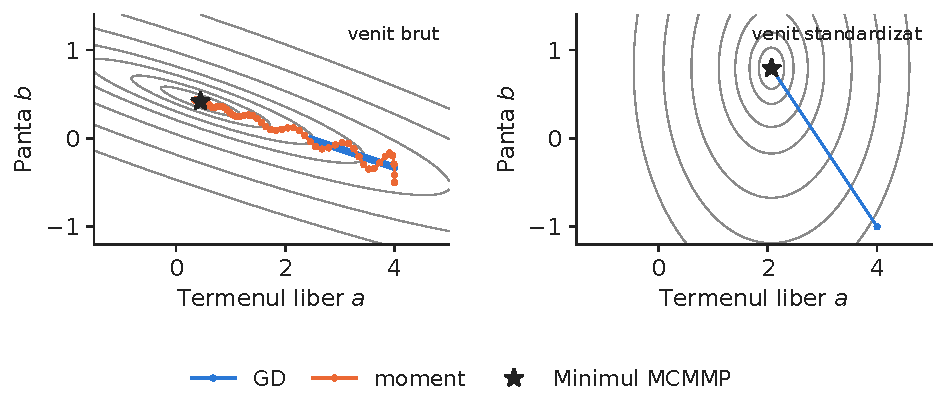
\includegraphics[width=\textwidth,height=0.280\textheight,keepaspectratio]{charts/ro/gd_paths.pdf}\end{center}\vspace{-3mm}
\chartsource{Sursa: StatLib, locuințe din California, recensămîntul din 1990 (Pace și Barry, 1997). Date: 20\,640 de grupuri de locuințe\, recensămîntul din 1990.}
\vspace{0.5mm}
\begin{itemize}\setlength{\itemsep}{0pt}
  \item Numărul de condiționare $\kappa=\lambda_{\max}/\lambda_{\min}$ al hessianei: 104{,}3 brut, 1 standardizat
    \begin{itemize}\setlength{\itemsep}{0pt}
      \item După 60 de pași: eroarea pătratică medie (MSE) 1{,}486 (GD, brut), 0{,}704 (moment, brut), 0{,}701 (GD, standardizat)
      \item Minimul 0{,}701.
    \end{itemize}
\end{itemize}
\par\vfill\manager{standardizați fiecare intrare pe setul de antrenare înainte de a antrena orice rețea.}\par\vspace{0.5mm}
\par\vfill\noindent{\scriptsize\color{FooterGray}(calcul propriu)}\hfill\qlink{NN\_L2\_gd\_paths}{Quantlets/L2/NN_L2_gd_paths}\par\vspace{0.5mm}
\end{frame}

\begin{frame}{Pe o funcție pătratică, pasul trebuie să rămînă sub $2/\lambda_{\max}$}
\small
\intuition{pe fiecare direcție proprie a hessianei, coborîrea pe gradient înmulțește eroarea cu $(1-\eta\lambda_k)$.}
\[ \loss(\btheta)=\loss^*+\tfrac12(\btheta-\btheta^*)^\top\mathbf H(\btheta-\btheta^*)\ \Rightarrow\ \btheta_{t}-\btheta^*=(\mathbf I-\eta\mathbf H)^t(\btheta_0-\btheta^*),\qquad |1-\eta\lambda_k|<1\iff 0<\eta<\frac{2}{\lambda_{\max}} \]
{\footnotesize\begin{itemize}\setlength{\itemsep}{0pt}
  \item \textbf{\txtwhere}
    \begin{itemize}\setlength{\itemsep}{0pt}
      \item $\mathbf H$ hessiana, cu valorile proprii $\lambda_{\min}\le\dots\le\lambda_{\max}$, $\btheta^*$ minimul
    \end{itemize}
\end{itemize}\par}
\begin{itemize}\setlength{\itemsep}{2pt}
  \item Cu cel mai bun pas fix, eroarea scade cu factorul $(\kappa-1)/(\kappa+1)$ la fiecare pas: lent cînd $\kappa$ este mare.
  \item Venitul brut: $\kappa=$ 104{,}3, deci pasul $1/\lambda_{\max}=$ 0{,}0258 abia mișcă direcția plată.
  \item Rețelele nu sînt pătratice, dar lîngă un minim se comportă ca una: aceeași limită explică divergența la $\eta$ mare.
\end{itemize}
\par\vfill\manager{dacă pierderea explodează în primele epoci, împărțiți rata de învățare la 3 înainte de a schimba altceva.}\par\vspace{0.5mm}
\par\vfill\noindent{\scriptsize\color{FooterGray}(Bishop \& Bishop, 2024, ch.~7)}\par\vspace{0.5mm}
\end{frame}


\section{Propagarea înapoi a erorii}

\begin{frame}{Propagarea înapoi este regula de derivare a funcțiilor compuse, aplicată de la pierdere înapoi}
\small
\intuition{fiecare nod al grafului de calcul înmulțește gradientul primit cu propria derivată locală și îl transmite mai departe.}
\[ \vz^{(l)}=\mW^{(l)}\vh^{(l-1)}+\vb^{(l)},\quad \vh^{(l)}=a(\vz^{(l)});\qquad \boldsymbol\delta^{(L)}=\frac{\partial\ell}{\partial\vz^{(L)}},\quad \boldsymbol\delta^{(l)}=\big(\mW^{(l+1)\top}\boldsymbol\delta^{(l+1)}\big)\odot a'(\vz^{(l)}) \]
\[ \frac{\partial\ell}{\partial\mW^{(l)}}=\boldsymbol\delta^{(l)}\,\vh^{(l-1)\top},\qquad \frac{\partial\ell}{\partial\vb^{(l)}}=\boldsymbol\delta^{(l)} \]
{\footnotesize\begin{itemize}\setlength{\itemsep}{0pt}
  \item \textbf{\txtwhere}
    \begin{itemize}\setlength{\itemsep}{0pt}
      \item $\boldsymbol\delta^{(l)}$ semnalul de eroare al stratului $l$, $\odot$ produsul element cu element, $a'$ derivata funcției de activare
    \end{itemize}
\end{itemize}\par}
\begin{itemize}\setlength{\itemsep}{2pt}
  \item Eroarea de ieșire: $\hat y-y$ (pierdere pătratică), $p-y$ (sigmoidă cu entropie încrucișată, cursul 1).
  \item Gradientul unei ponderi = eroarea stratului înmulțită cu intrarea lui, ca la gradientul logistic.
\end{itemize}
\par\vfill\manager{propagarea înainte trebuie să rețină $\vz^{(l)}$ și $\vh^{(l)}$: memoria, nu calculul, limitează mărimea lotului pe un procesor grafic (GPU).}\par\vspace{0.5mm}
\par\vfill\noindent{\scriptsize\color{FooterGray}(Rumelhart, Hinton \& Williams, 1986)}\par\vspace{0.5mm}
\end{frame}

\begin{frame}{Propagarea înapoi, de mînă, pentru un grup real de locuințe}
\small
\intuition{două intrări standardizate, două unități liniare rectificate (ReLU), ieșire liniară, $\ell=\tfrac12(\hat y-y)^2$.}
\begin{columns}[T,onlytextwidth]
\begin{column}{0.48\textwidth}
{\scriptsize\renewcommand{\arraystretch}{1.05}\setlength{\tabcolsep}{4pt}
\begin{tabular}{@{}lrr@{}}\toprule
Înainte & neuronul 1 & neuronul 2 \\ \midrule
intrarea $x$ (venit, latitudine) & \ensuremath{-}0{,}21 & \ensuremath{-}0{,}67 \\
ponderile $\mW^{(1)}$, rîndul 1 / 2 & \ensuremath{-}0{,}28, \ensuremath{-}0{,}56 & 0{,}50, \ensuremath{-}0{,}02 \\
$z=\mW^{(1)}x$ & 0{,}433 & \ensuremath{-}0{,}093 \\
$h=\max(0,z)$ & 0{,}433 & 0{,}000 \\
ponderile de ieșire $w^{(2)}$ & \ensuremath{-}0{,}87 & \ensuremath{-}0{,}19 \\
$\hat y=w^{(2)\top}h$; $y$ & \ensuremath{-}0{,}377 & 2{,}067 \\
\bottomrule\end{tabular}}
\end{column}
\begin{column}{0.49\textwidth}
{\scriptsize\renewcommand{\arraystretch}{1.05}\setlength{\tabcolsep}{4pt}
\begin{tabular}{@{}lrr@{}}\toprule
Înapoi & neuronul 1 & neuronul 2 \\ \midrule
$\delta^{(2)}=\hat y-y$ & \ensuremath{-}2{,}444 &  \\
$\partial\ell/\partial w^{(2)}=\delta^{(2)}h$ & \ensuremath{-}1{,}059 & \ensuremath{-}0{,}000 \\
$\delta^{(1)}=\delta^{(2)}w^{(2)}\odot\mathbb 1\{z>0\}$ & 2{,}126 & 0{,}000 \\
$\partial\ell/\partial W^{(1)}_{k1}=\delta^{(1)}_kx_1$ & \ensuremath{-}0{,}453 & \ensuremath{-}0{,}000 \\
$\partial\ell/\partial W^{(1)}_{k2}=\delta^{(1)}_kx_2$ & \ensuremath{-}1{,}419 & \ensuremath{-}0{,}000 \\
\bottomrule\end{tabular}}
\end{column}
\end{columns}\begin{itemize}\setlength{\itemsep}{2pt}
  \item Neuronul 2 este oprit ($z_2<0$): nu transmite gradient, deci ponderile lui nu se modifică.
  \item Diferențierea automată din PyTorch dă aceiași gradienți (diferența maximă 0{,}0).
\end{itemize}
\par\vfill\manager{un neuron ReLU oprit pentru toți clienții nu mai învață niciodată: urmăriți ponderea neuronilor „morți”.}\par\vspace{0.5mm}
\par\vfill\noindent{\scriptsize\color{FooterGray}(calcul propriu)}\hfill\tryit{notebook \S2}\par\vspace{0.5mm}
\end{frame}

\begin{frame}{Modul invers costă cam încă o propagare înainte, oricîte ponderi ar fi}
\small
\intuition{o singură trecere înapoi dă toate cele $P$ derivate parțiale ale unei pierderi scalare; diferențele finite ar cere $P$ treceri în plus.}
\[ \text{cost}\big(\nabla_{\btheta}\loss\big)\ \le\ c\cdot\text{cost}\big(\loss\big),\ \ c\approx 2\text{--}3;\qquad \frac{\partial\loss}{\partial\theta_j}\approx\frac{\loss(\btheta+\epsilon\mathbf e_j)-\loss(\btheta-\epsilon\mathbf e_j)}{2\epsilon} \]
\begin{itemize}\setlength{\itemsep}{2pt}
  \item Modul direct (numere duale) este ieftin pentru puține intrări și multe ieșiri
    \begin{itemize}\setlength{\itemsep}{0pt}
      \item Modul invers pentru multe intrări (ponderi) și o ieșire (pierderea).
    \end{itemize}
  \item Verificarea gradientului pe MLP 64-64: 30 de ponderi alese aleator, diferențe centrale cu $\epsilon=10^{-6}$ în dublă precizie, eroarea relativă maximă $7{,}0\times10^{-7}$.
  \item PyTorch înregistrează graful în timpul propagării înainte
    \begin{itemize}\setlength{\itemsep}{0pt}
      \item \texttt{loss.backward()} îl parcurge invers.
    \end{itemize}
\end{itemize}
\par\vfill\manager{cînd scrieți un strat sau o pierdere proprie, rulați o dată verificarea gradientului înainte de a vă baza pe ele.}\par\vspace{0.5mm}
\par\vfill\noindent{\scriptsize\color{FooterGray}(Baydin et al., 2018; Paszke et al., 2019)}\hfill\tryit{notebook \S2}\par\vspace{0.5mm}
\end{frame}

\begin{frame}{Dispariția gradientului în rețelele adînci cu activare sigmoidă}
\small
\intuition{semnalul înapoi este un produs de matrice jacobiene; cu $\sigma'\le1/4$, el scade la fiecare strat.}
\vspace{-1mm}\[ \frac{\partial\ell}{\partial\vh^{(l)}}=\Big(\prod_{k=l+1}^{L}\mW^{(k)\top}\operatorname{diag}\big(a'(\vz^{(k)})\big)\Big)\frac{\partial\ell}{\partial\vh^{(L)}} \]\vspace{-2mm}
\begin{center}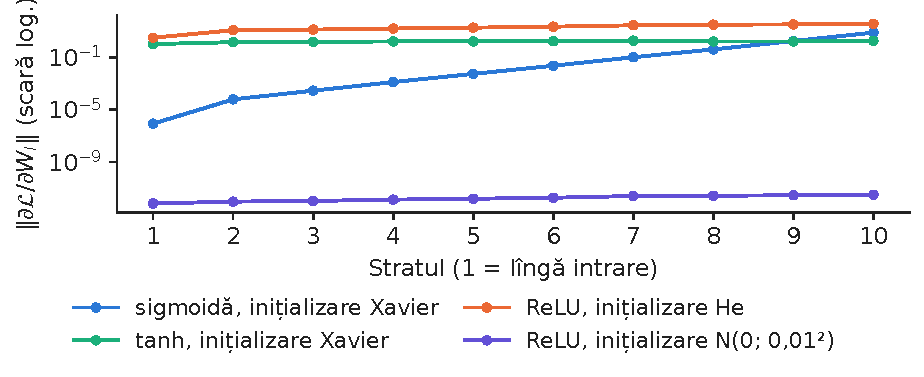
\includegraphics[width=\textwidth,height=0.271\textheight,keepaspectratio]{charts/ro/vanishing.pdf}\end{center}\vspace{-3mm}
\chartsource{Sursa: StatLib, locuințe din California, recensămîntul din 1990 (Pace și Barry, 1997). Date: 10 straturi ascunse de 64 de neuroni, un lot de 512 grupuri de antrenare, 5 inițializări.}
\vspace{0.5mm}
\begin{itemize}\setlength{\itemsep}{0pt}
  \item 10 straturi ascunse, un lot real: norma gradientului în primul/ultimul strat $8{,}5\times10^{-7}$ față de $7{,}5\times10^{0}$ cu sigmoide
    \begin{itemize}\setlength{\itemsep}{0pt}
      \item $3{,}1\times10^{0}$ față de $3{,}5\times10^{1}$ cu ReLU și inițializare He.
    \end{itemize}
\end{itemize}
\par\vfill\manager{rețelele adînci au nevoie de activări ReLU, de o inițializare scalată și de normalizare (cursul 3).}\par\vspace{0.5mm}
\par\vfill\noindent{\scriptsize\color{FooterGray}(calcul propriu)}\hfill\qlink{NN\_L2\_vanishing}{Quantlets/L2/NN_L2_vanishing}\par\vspace{0.5mm}
\end{frame}

\begin{frame}{Inițializarea păstrează constantă varianța semnalului între straturi}
\small
\intuition{prea mică și semnalul dispare, prea mare și explodează; scara depinde de numărul de intrări și de activare.}
\[ \Var(z_j^{(l)})=n_{l-1}\Var(W)\,\E\big[(h^{(l-1)})^2\big]\ \Rightarrow\ \underbrace{\Var(W)=\frac{2}{n_{l-1}+n_l}}_{\text{Xavier (tanh, sigmoid)}},\qquad \underbrace{\Var(W)=\frac{2}{n_{l-1}}}_{\text{He (ReLU)}} \]
{\footnotesize\begin{itemize}\setlength{\itemsep}{0pt}
  \item \textbf{\txtwhere}
    \begin{itemize}\setlength{\itemsep}{0pt}
      \item $n_{l-1}$ numărul de intrări, $n_l$ numărul de ieșiri ale stratului $l$, pentru ReLU, $\E[h^2]=\tfrac12\Var(z)$, de unde factorul 2
    \end{itemize}
\end{itemize}\par}
\begin{itemize}\setlength{\itemsep}{2pt}
  \item Ponderi $\mathcal N(0;0{,}01^2)$, rețea ReLU cu 10 straturi: norma gradientului în primul strat $6{,}9\times10^{-13}$, deci nicio învățare.
  \item Nu inițializați toate ponderile la fel: toți neuronii ar învăța același lucru.
\end{itemize}
\par\vfill\manager{valorile implicite din PyTorch sînt apropiate de aceste reguli
    \begin{itemize}\setlength{\itemsep}{0pt}
      \item Pentru rețele ReLU adînci, setați explicit inițializarea He.
    \end{itemize}}\par\vspace{0.5mm}
\par\vfill\noindent{\scriptsize\color{FooterGray}(Glorot \& Bengio, 2010; He et al., 2015)}\hfill\tryit{notebook \S3}\par\vspace{0.5mm}
\end{frame}


\section{Optimizarea stohastică}

\begin{frame}{Un mini-lot dă un gradient nedeplasat și zgomotos, la o fracțiune din cost}
\small
\intuition{media gradientului pe $B$ exemple aleatoare este suficientă pentru a ști aproximativ încotro este coborîrea.}
\[ \mathbf g_t=\frac1B\sum_{i\in\mathcal B_t}\nabla\ell_i(\btheta_t),\qquad \E[\mathbf g_t]=\nabla\loss(\btheta_t),\qquad \Var(\mathbf g_t)\approx\frac{1}{B}\Big(1-\frac{B}{n}\Big)\Sigma(\btheta_t) \]
{\footnotesize\begin{itemize}\setlength{\itemsep}{0pt}
  \item \textbf{\txtwhere}
    \begin{itemize}\setlength{\itemsep}{0pt}
      \item $\mathcal B_t$ un lot aleator de mărime $B$, $\Sigma$ covarianța gradienților pe exemple, o epocă $=\lceil n/B\rceil$ pași
    \end{itemize}
\end{itemize}\par}
\begin{itemize}\setlength{\itemsep}{2pt}
  \item Robbins--Monro: cu $\sum_t\eta_t=\infty$ și $\sum_t\eta_t^2<\infty$, SGD converge către un punct staționar.
  \item Zgomotul nu este doar un cost: ajută la ieșirea din minimele abrupte, care tind să generalizeze mai slab (Keskar et al., 2017).
\end{itemize}
\par\vfill\manager{loturile de 32--256 de exemple sînt compromisul obișnuit între zgomot, viteză și memorie.}\par\vspace{0.5mm}
\par\vfill\noindent{\scriptsize\color{FooterGray}(Robbins \& Monro, 1951)}\hfill\tryit{notebook \S4}\par\vspace{0.5mm}
\end{frame}

\begin{frame}{Efectul ratei de învățare asupra antrenării}
\small
\intuition{SGD simplu pe un MLP 64-64, 30 de epoci, loturi de 128, pentru nouă rate de învățare și trei inițializări.}
\begin{center}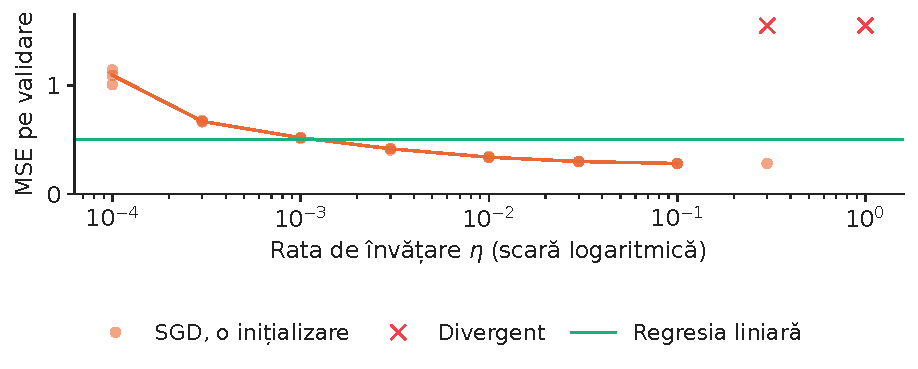
\includegraphics[width=\textwidth,height=0.389\textheight,keepaspectratio]{charts/ro/lr_sweep.pdf}\end{center}\vspace{-3mm}
\chartsource{Sursa: StatLib, locuințe din California, recensămîntul din 1990 (Pace și Barry, 1997). Date: 12\,384 de grupuri de antrenare și 4\,128 de validare; 30 de epoci.}
\vspace{0.5mm}
\begin{itemize}\setlength{\itemsep}{0pt}
  \item MSE pe validare 1{,}093 la $\eta=10^{-4}$ (mai slab decît regresia liniară, 0{,}500), 0{,}281 la $\eta=$ 0{,}1
    \begin{itemize}\setlength{\itemsep}{0pt}
      \item De la $\eta=$ 0{,}3, cel puțin o inițializare diverge.
    \end{itemize}
\end{itemize}
\par\vfill\manager{ajustați mai întîi rata de învățare, pe o grilă logaritmică, înaintea oricărui alt hiperparametru.}\par\vspace{0.5mm}
\par\vfill\noindent{\scriptsize\color{FooterGray}(calcul propriu)}\hfill\qlink{NN\_L2\_lr\_sweep}{Quantlets/L2/NN_L2_lr_sweep}\par\vspace{0.5mm}
\end{frame}

\begin{frame}{Efectul dimensiunii lotului: progresul pe epocă și pe secundă}
\small
\intuition{Adam cu rata de învățare 0,001, 40 de epoci, loturi de 16, 128 și 1\,024 de exemple.}
\begin{center}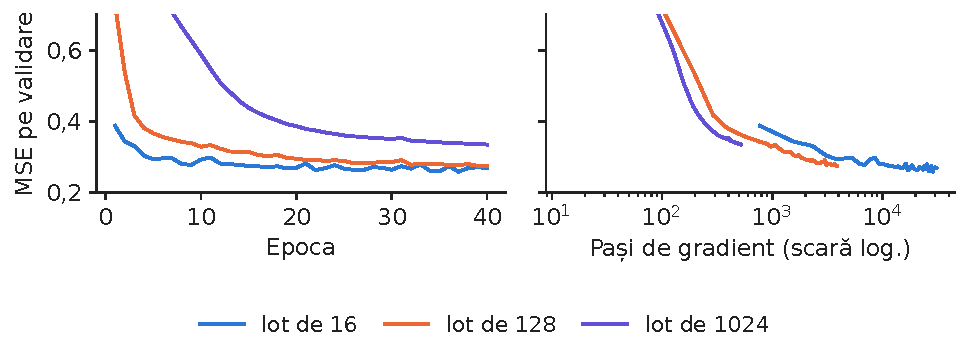
\includegraphics[width=\textwidth,height=0.437\textheight,keepaspectratio]{charts/ro/batch_size.pdf}\end{center}\vspace{-3mm}
\chartsource{Sursa: StatLib, locuințe din California, recensămîntul din 1990 (Pace și Barry, 1997). Date: Adam, rata de învățare 0,001, 40 de epoci.}
\vspace{0.5mm}
\begin{itemize}\setlength{\itemsep}{0pt}
  \item După 5 epoci: MSE pe validare 0{,}294 (lot 16), 0{,}367 (128), 0{,}870 (1\,024)
    \begin{itemize}\setlength{\itemsep}{0pt}
      \item Durata a 40 de epoci pe un fir al procesorului: 25{,}8, 3{,}7 și 1{,}0 secunde.
    \end{itemize}
\end{itemize}
\par\vfill\manager{comparați bugetele de antrenare în pași de gradient sau în secunde, nu în epoci.}\par\vspace{0.5mm}
\par\vfill\noindent{\scriptsize\color{FooterGray}(calcul propriu)}\hfill\qlink{NN\_L2\_batch\_size}{Quantlets/L2/NN_L2_batch_size}\par\vspace{0.5mm}
\end{frame}

\begin{frame}{Metoda momentului: media mobilă a gradienților trecuți}
\small
\intuition{componentele în zigzag se anulează în medie, iar componenta constantă spre vale se acumulează.}
\[ \mathbf v_{t+1}=\beta\,\mathbf v_t+\mathbf g_t,\qquad \btheta_{t+1}=\btheta_t-\eta\,\mathbf v_{t+1};\qquad \text{Nesterov:}\ \mathbf g_t=\nabla\loss(\btheta_t-\eta\beta\mathbf v_t) \]
{\footnotesize\begin{itemize}\setlength{\itemsep}{0pt}
  \item \textbf{\txtwhere}
    \begin{itemize}\setlength{\itemsep}{0pt}
      \item $\mathbf v$ viteza, $\beta\in[0,1)$ coeficientul de moment, de obicei 0,9, pe o pantă constantă, pasul efectiv este $\eta/(1-\beta)$, de zece ori $\eta$
    \end{itemize}
\end{itemize}\par}
\begin{itemize}\setlength{\itemsep}{2pt}
  \item Pe o funcție pătratică, momentul optim îmbunătățește contracția de la $\frac{\kappa-1}{\kappa+1}$ la $\frac{\sqrt\kappa-1}{\sqrt\kappa+1}$ (Polyak, 1964).
  \item Regresia pe venitul brut după 60 de pași: MSE 0{,}704 cu moment, față de 1{,}486 pentru GD simplu.
\end{itemize}
\par\vfill\manager{SGD cu moment 0,9 rămîne alegerea implicită pentru modelele foarte mari de vedere artificială.}\par\vspace{0.5mm}
\par\vfill\noindent{\scriptsize\color{FooterGray}(Polyak, 1964)}\hfill\tryit{notebook \S5}\par\vspace{0.5mm}
\end{frame}

\begin{frame}{Metodele adaptive dau fiecărei ponderi propriul pas}
\small
\intuition{împărțiți pasul la o măsură curentă a mărimii gradienților acelei ponderi.}
\[ \text{AdaGrad: } s_t=s_{t-1}+g_t^2;\qquad \text{RMSProp: } s_t=\rho\,s_{t-1}+(1-\rho)\,g_t^2;\qquad \theta_{t+1}=\theta_t-\frac{\eta}{\sqrt{s_t}+\epsilon}\,g_t \]
{\footnotesize\begin{itemize}\setlength{\itemsep}{0pt}
  \item \textbf{\txtwhere}
    \begin{itemize}\setlength{\itemsep}{0pt}
      \item Toate operațiile element cu element, $\rho\approx0{,}99$, $\epsilon\approx10^{-8}$ evită împărțirea la zero
    \end{itemize}
\end{itemize}\par}
\begin{itemize}\setlength{\itemsep}{2pt}
  \item Suma din AdaGrad doar crește, deci pașii lui scad spre zero: bun pentru variabile rare, prea lent pentru rețele adînci (Duchi, Hazan \& Singer, 2011).
  \item Propagarea cu medie pătratică (RMSProp) uită exponențial gradienții vechi, deci pasul se adaptează regiunii curente (Tieleman \& Hinton, 2012).
  \item Rescalarea pe fiecare pondere compensează parțial condiționarea proastă: direcțiile plate sau rar actualizate primesc pași mai mari.
\end{itemize}
\par\vfill\manager{metodele adaptive sînt mai puțin sensibile la rata de învățare, ceea ce le face o primă alegere sigură.}\par\vspace{0.5mm}
\par\vfill\noindent{\scriptsize\color{FooterGray}}\hfill\tryit{notebook \S5}\par\vspace{0.5mm}
\end{frame}

\begin{frame}{Adam = moment + RMSProp + o corecție a deplasării}
\small
\intuition{păstrăm medii mobile ale gradientului și ale pătratului lui, le corectăm pentru pornirea de la zero și facem un pas egal cu raportul lor.}
\[ m_t=\beta_1m_{t-1}+(1-\beta_1)g_t,\quad v_t=\beta_2v_{t-1}+(1-\beta_2)g_t^2,\quad \hat m_t=\frac{m_t}{1-\beta_1^t},\ \hat v_t=\frac{v_t}{1-\beta_2^t},\quad \theta_{t+1}=\theta_t-\eta\,\frac{\hat m_t}{\sqrt{\hat v_t}+\epsilon} \]
{\footnotesize\begin{itemize}\setlength{\itemsep}{0pt}
  \item \textbf{\txtwhere}
    \begin{itemize}\setlength{\itemsep}{0pt}
      \item Valori implicite $\beta_1=0{,}9$, $\beta_2=0{,}999$, $\epsilon=10^{-8}$, $\eta=10^{-3}$, $m_0=v_0=0$, de unde corecția (anexa)
    \end{itemize}
\end{itemize}\par}
\begin{itemize}\setlength{\itemsep}{2pt}
  \item Pasul este aproximativ limitat la $\eta$ pentru fiecare pondere, oricare ar fi scara pierderii: ușor de ajustat.
  \item Adam cu penalizarea ponderilor decuplată (AdamW) micșorează direct ponderile, $\theta\leftarrow\theta-\eta\lambda\theta$, în loc să adauge $\lambda\theta$ la $g_t$ (Loshchilov \& Hutter, 2019; cursul 3).
\end{itemize}
\par\vfill\manager{porniți de la AdamW cu $\eta=10^{-3}$
    \begin{itemize}\setlength{\itemsep}{0pt}
      \item Treceți la SGD cu moment, ajustat, doar dacă cîștigați în afara eșantionului.
    \end{itemize}}\par\vspace{0.5mm}
\par\vfill\noindent{\scriptsize\color{FooterGray}(Kingma \& Ba, 2015)}\hfill\tryit{notebook \S5}\par\vspace{0.5mm}
\end{frame}

\begin{frame}{Pe datele California, toți optimizatorii ajustați ajung aproape; cei adaptivi ajung mai sigur}
\small
\intuition{cea mai bună dintre trei rate de învățare (pe validare), media a 5 inițializări noi.}
\begin{center}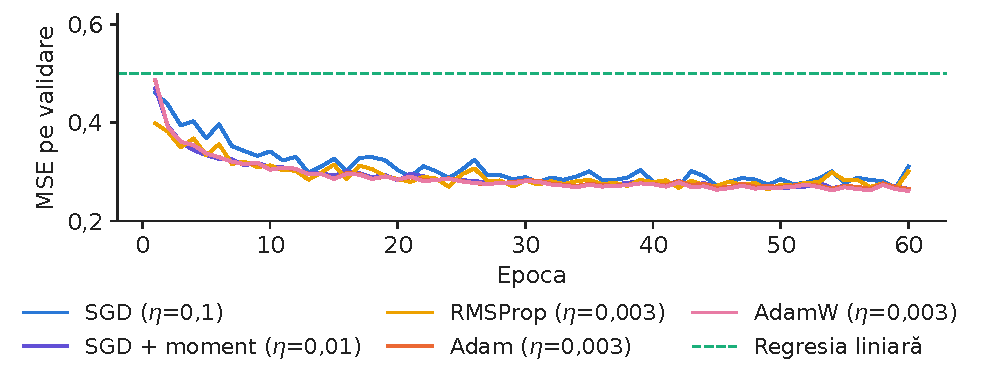
\includegraphics[width=\textwidth,height=0.304\textheight,keepaspectratio]{charts/ro/optimizers.pdf}\end{center}\vspace{-3mm}
\chartsource{Sursa: StatLib, locuințe din California, recensămîntul din 1990 (Pace și Barry, 1997). Date: 12\,384 de grupuri de antrenare și 4\,128 de validare.}
\vspace{0.5mm}
\begin{itemize}\setlength{\itemsep}{0pt}
  \item MSE pe validare după 10 epoci: SGD 0{,}342, moment 0{,}310, RMSProp 0{,}313, Adam 0{,}305, AdamW 0{,}304
    \begin{itemize}\setlength{\itemsep}{0pt}
      \item Regresia liniară 0{,}500.
    \end{itemize}
\end{itemize}
\par\vfill\manager{rețeaua înjumătățește eroarea modelului liniar de referință, oricare ar fi optimizatorul.}\par\vspace{0.5mm}
\par\vfill\noindent{\scriptsize\color{FooterGray}(calcul propriu)}\hfill\qlink{NN\_L2\_optimizers}{Quantlets/L2/NN_L2_optimizers}\par\vspace{0.5mm}
\end{frame}

\begin{frame}{De la o inițializare la alta, Adam și AdamW sînt mult mai stabile decît SGD simplu}
\small
\intuition{MSE pe test pentru 5 inițializări la fiecare optimizator; o singură rulare le-ar fi ordonat la întîmplare.}
\begin{center}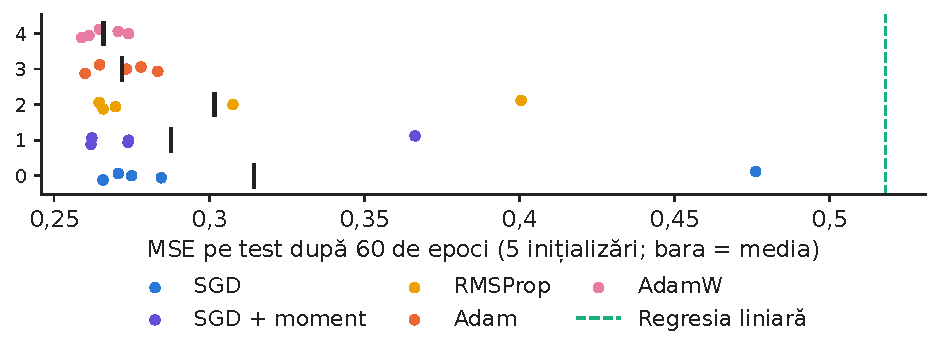
\includegraphics[width=\textwidth,height=0.257\textheight,keepaspectratio]{charts/ro/optimizer_seeds.pdf}\end{center}\vspace{-3mm}
\chartsource{Sursa: StatLib, locuințe din California, recensămîntul din 1990 (Pace și Barry, 1997). Date: 4\,128 de grupuri de testare.}
\vspace{0.5mm}
\begin{itemize}\setlength{\itemsep}{0pt}
  \item MSE pe test, media (abaterea standard): SGD 0{,}314 (0{,}091), Adam 0{,}272 (0{,}010), AdamW 0{,}266 (0{,}006)
    \begin{itemize}\setlength{\itemsep}{0pt}
      \item Testul $t$ pe perechi SGD față de Adam: $t=$ 1{,}01, $p=$ 0{,}371.
    \end{itemize}
\end{itemize}
\par\vfill\manager{cîștigul mediu nu este semnificativ cu 5 inițializări, dar riscul unei rulări proaste este mult mai mic cu Adam.}\par\vspace{0.5mm}
\par\vfill\noindent{\scriptsize\color{FooterGray}(calcul propriu)}\hfill\qlink{NN\_L2\_optimizer\_seeds}{Quantlets/L2/NN_L2_optimizer_seeds}\par\vspace{0.5mm}
\end{frame}

\begin{frame}{Programele ratei de învățare: în trepte, cosinus și one-cycle}
\small
\intuition{explorăm cu un pas mare, apoi îl reducem, ca zgomotul SGD să se așeze într-un minim.}
\[ \text{trepte: }\eta_t=\eta_0\gamma^{\lfloor t/s\rfloor};\qquad \text{cosinus: }\eta_t=\tfrac{\eta_0}{2}\Big(1+\cos\frac{\pi t}{T}\Big) \]
\[ \text{un ciclu: creștere liniară pînă la }\eta_0,\text{ apoi cosinus spre }\approx0 \]
{\footnotesize\begin{itemize}\setlength{\itemsep}{0pt}
  \item \textbf{\txtwhere}
    \begin{itemize}\setlength{\itemsep}{0pt}
      \item $\eta_0$ rata maximă, $\gamma$ factorul de scădere la fiecare $s$ pași, $T$ numărul total de pași
    \end{itemize}
\end{itemize}\par}
\begin{itemize}\setlength{\itemsep}{2pt}
  \item Descreșterea cosinus (Loshchilov \& Hutter, 2017) și programul cu un singur ciclu (Smith \& Topin, 2019) au nevoie doar de rata maximă și de buget.
  \item Încălzirea protejează primii pași, cînd estimările momentului al doilea din Adam și statisticile loturilor nu sînt încă fiabile.
\end{itemize}
\par\vfill\manager{un program cosinus pe numărul planificat de epoci este o alegere implicită sigură.}\par\vspace{0.5mm}
\par\vfill\noindent{\scriptsize\color{FooterGray}(Bishop \& Bishop, 2024, ch.~7)}\hfill\tryit{notebook \S6}\par\vspace{0.5mm}
\end{frame}

\begin{frame}{Scăderea ratei de învățare reduce eroarea finală}
\small
\intuition{SGD cu moment 0,9 și rata maximă 0,01; stînga: programele, dreapta: MSE pe validare (media a 3 inițializări).}
\begin{center}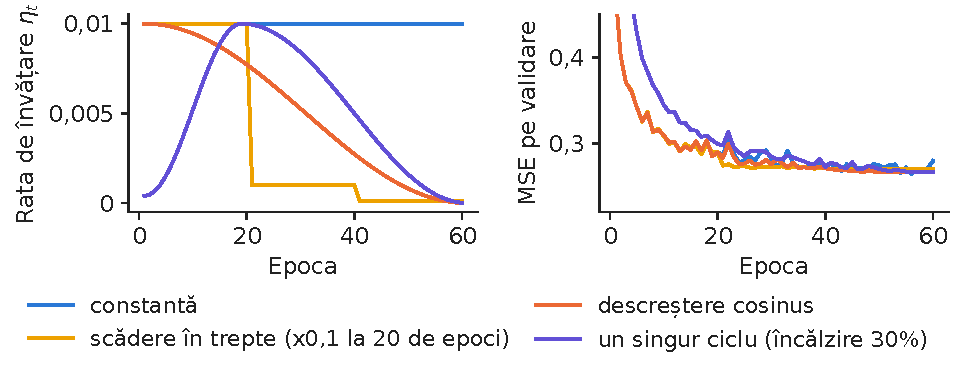
\includegraphics[width=\textwidth,height=0.385\textheight,keepaspectratio]{charts/ro/schedules.pdf}\end{center}\vspace{-3mm}
\chartsource{Sursa: StatLib, locuințe din California, recensămîntul din 1990 (Pace și Barry, 1997). Date: SGD cu moment 0,9, rata maximă 0,01, 3 inițializări.}
\vspace{0.5mm}
\begin{itemize}\setlength{\itemsep}{0pt}
  \item MSE final pe validare: constantă 0{,}279, trepte 0{,}270, cosinus 0{,}266, un ciclu 0{,}266
    \begin{itemize}\setlength{\itemsep}{0pt}
      \item Pe test 0{,}286 față de 0{,}265 (constantă față de cosinus).
    \end{itemize}
\end{itemize}
\par\vfill\manager{programul ratei este un cîștig ieftin: același model, același buget, eroare mai mică.}\par\vspace{0.5mm}
\par\vfill\noindent{\scriptsize\color{FooterGray}(calcul propriu)}\hfill\qlink{NN\_L2\_schedules}{Quantlets/L2/NN_L2_schedules}\par\vspace{0.5mm}
\end{frame}

\begin{frame}{La fraudele cu carduri, optimizatorul determină viteza învățării}
\small
\intuition{MLP 64-64 antrenat pe primele 60\,\% din cele două zile, evaluat pe următoarele 20\,\%.}
\begin{center}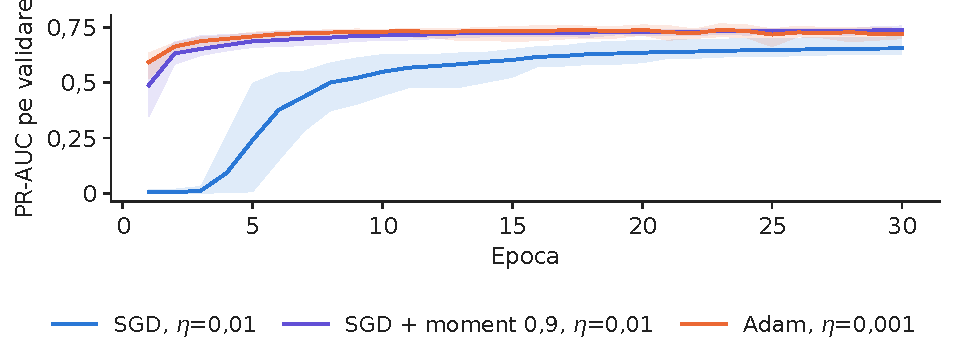
\includegraphics[width=\textwidth,height=0.414\textheight,keepaspectratio]{charts/ro/fraud_optimizers.pdf}\end{center}\vspace{-3mm}
\chartsource{Sursa: ULB Machine Learning Group și Worldline, tranzacții cu carduri (OpenML 1597). Date: septembrie 2013, 2 zile; antrenare = primele 33,4 ore, validare pînă la ora 40,3; 5 inițializări.}
\vspace{0.5mm}
\begin{itemize}\setlength{\itemsep}{0pt}
  \item Aria de sub curba precizie-sensibilitate (PR-AUC) după o epocă: SGD 0{,}004, moment 0{,}488, Adam 0{,}592 (orele de test: 0{,}786, 0{,}823, 0{,}803).
\end{itemize}
\par\vfill\manager{cu o clasă rară, SGD simplu are nevoie de multe epoci, momentul sau Adam de una singură.}\par\vspace{0.5mm}
\par\vfill\noindent{\scriptsize\color{FooterGray}(calcul propriu)}\hfill\qlink{NN\_L2\_fraud\_optimizers}{Quantlets/L2/NN_L2_fraud_optimizers}\par\vspace{0.5mm}
\end{frame}

\begin{frame}{Compararea optimizatorilor}
\small
{\scriptsize\renewcommand{\arraystretch}{1.05}\setlength{\tabcolsep}{4pt}
\begin{tabular}{@{}p{0.15\textwidth}p{0.37\textwidth}p{0.17\textwidth}p{0.24\textwidth}@{}}\toprule
Metoda & Actualizarea & Memorie suplimentară & Cînd se folosește \\ \midrule
SGD & $\theta-\eta g$ & nimic & modele mari de imagini, program ajustat \\
Moment & $v\leftarrow\beta v+g$, $\theta-\eta v$ & 1 vector & pierderi prost condiționate \\
RMSProp & $\theta-\eta g/\sqrt{s}$, $s$ = medie$(g^2)$ & 1 vector & rețele recurente, pierderi nestaționare \\
Adam & $\theta-\eta\hat m/(\sqrt{\hat v}+\epsilon)$ & 2 vectori & prima alegere implicită \\
AdamW & Adam $+$ micșorare $(1-\eta\lambda)\theta$ & 2 vectori & ori de cîte ori se folosește penalizarea \\
\bottomrule\end{tabular}}
\par\vspace{0.5mm}{\scriptsize \begin{itemize}\setlength{\itemsep}{0pt}
  \item Memoria este pe pondere: Adam reține două numere suplimentare pentru fiecare parametru, ceea ce contează la modelele foarte mari.
\end{itemize}}
\par\vfill\manager{alegeți după buget și stabilitate
    \begin{itemize}\setlength{\itemsep}{0pt}
      \item Pe datele noastre, optimizatorii ajustați ajung aproape, iar Adam și AdamW sînt cei mai stabili.
    \end{itemize}}\par\vspace{0.5mm}
\par\vfill\noindent{\scriptsize\color{FooterGray}(Bishop \& Bishop, 2024, ch.~7)}\par\vspace{0.5mm}
\end{frame}


\section{Studiu de caz: valoarea la risc cu o rețea cuantilică}

\begin{frame}{Pierderea pinball transformă orice rețea într-un model de prognoză a cuantilelor}
\small
\intuition{penalizăm randamentele de sub prognoză de $(1-\tau)/\tau$ ori mai mult decît pe cele de deasupra, iar minimul este cuantila $\tau$.}
\[ \mathrm{VaR}^{\tau}_{t+1}=-q_{\tau}(r_{t+1}\mid\mathcal F_t),\qquad \rho_\tau(u)=u\big(\tau-\mathbb 1\{u<0\}\big),\qquad \hat q=\argmin_{q}\ \E\,\rho_\tau(r-q) \]
{\footnotesize\begin{itemize}\setlength{\itemsep}{0pt}
  \item \textbf{\txtwhere}
    \begin{itemize}\setlength{\itemsep}{0pt}
      \item $r_{t+1}$ randamentul logaritmic de a doua zi, în \%, $\mathcal F_t$ informația pînă în ziua $t$, $\tau=1\,\%$ pentru un VaR de 99\,\%
    \end{itemize}
\end{itemize}\par}
\begin{itemize}\setlength{\itemsep}{2pt}
  \item Rețeaua: intrări $r_t$, $|r_t|$, media pe 5 zile, volatilitatea pe 5, 22 și 66 de zile
    \begin{itemize}\setlength{\itemsep}{0pt}
      \item MLP 32-32 antrenat cu Adam pe $\frac1n\sum\rho_\tau(r_{t+1}-\hat q_t)$.
    \end{itemize}
  \item Antrenare de la 8 aprilie 2005 pînă în 2016, validare 2017--2019 pentru oprirea timpurie, test 3 ianuarie 2020 -- 30 octombrie 2026
    \begin{itemize}\setlength{\itemsep}{0pt}
      \item Media a 5 inițializări.
    \end{itemize}
  \item Modele de referință: simularea istorică pe 250 de zile și volatilitatea calculată cu media mobilă ponderată exponențial (EWMA), $\lambda=0{,}94$, cu cuantila normală.
\end{itemize}
\par\vfill\manager{aceeași rețea cu altă pierdere dă altă măsură de risc: pierderea definește ce se învață.}\par\vspace{0.5mm}
\par\vfill\noindent{\scriptsize\color{FooterGray}(Koenker \& Bassett, 1978)}\hfill\tryit{notebook \S8}\par\vspace{0.5mm}
\end{frame}

\begin{frame}{În pandemia din 2020 și după, VaR-ul MLP cuantilic este depășit aproximativ cît ar trebui}
\small
\intuition{doar perioada de test; punctele roșii sînt zilele în care S\&P 500 a pierdut mai mult decît VaR-ul de 99\,\% al MLP.}
\begin{center}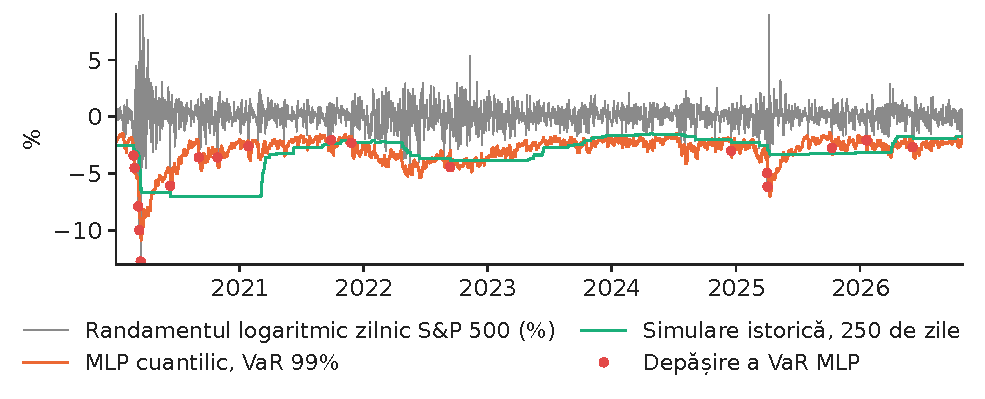
\includegraphics[width=\textwidth,height=0.370\textheight,keepaspectratio]{charts/ro/var_backtest.pdf}\end{center}\vspace{-3mm}
\chartsource{Sursa: Yahoo Finance, cotații zilnice. Date: 3 ianuarie 2020 - 30 octombrie 2026, zile de tranzacționare (perioada de test).}
\vspace{0.5mm}
\begin{itemize}\setlength{\itemsep}{0pt}
  \item Depășiri pe 1\,716 de zile (așteptat 17{,}2): MLP 18, simularea istorică 31, EWMA 41
    \begin{itemize}\setlength{\itemsep}{0pt}
      \item VaR mediu 2{,}96\,\%, 3{,}28\,\%, 2{,}52\,\%.
    \end{itemize}
\end{itemize}
\par\vfill\manager{un VaR care reacționează în cîteva zile la volatilitate evită grupările de depășiri ale simulării istorice.}\par\vspace{0.5mm}
\par\vfill\noindent{\scriptsize\color{FooterGray}(calcul propriu)}\hfill\qlink{NN\_L2\_var\_backtest}{Quantlets/L2/NN_L2_var_backtest}\par\vspace{0.5mm}
\end{frame}

\begin{frame}{Testul Kupiec acceptă MLP și respinge ambele modele de referință}
\small
\intuition{dacă VaR-ul este corect, numărul de depășiri este binomial, cu probabilitatea $\tau$; testăm rata observată față de ea.}
\[ \mathrm{LR}_{\mathrm{POF}}=-2\ln\frac{(1-\tau)^{n-x}\tau^{x}}{(1-\hat\pi)^{n-x}\hat\pi^{x}}\ \sim\ \chi^2_1,\quad \hat\pi=\frac xn,\ n\ \text{zile},\ x\ \text{depășiri} \]
{\footnotesize\renewcommand{\arraystretch}{1.05}\setlength{\tabcolsep}{4pt}
\begin{tabular}{@{}lrrrrr@{}}\toprule
Model & Depășiri & Rata (\%) & $\mathrm{LR}_{\mathrm{POF}}$ & $p$ & Pierderea pinball \\ \midrule
MLP cuantilic (5 inițializări) & 18 & 1{,}05 & 0{,}04 & 0{,}840 & 0{,}0420 \\
Simulare istorică, 250 de zile & 31 & 1{,}81 & 9{,}10 & 0{,}003 & 0{,}0577 \\
EWMA, $\lambda=0{,}94$ & 41 & 2{,}39 & 24{,}08 & 0{,}000 & 0{,}0473 \\
\bottomrule\end{tabular}}
\par\vspace{0.5mm}{\scriptsize \begin{itemize}\setlength{\itemsep}{0pt}
  \item Inițializările individuale dau rate de depășire între 1{,}05\,\% și 1{,}22\,\%; pierderea pinball este scorul potrivit pentru compararea prognozelor de cuantile.
\end{itemize}}
\par\vfill\manager{o autoritate de supraveghere se uită întîi la numărul de depășiri
    \begin{itemize}\setlength{\itemsep}{0pt}
      \item Un manager de risc ar trebui să compare și pierderile pinball.
    \end{itemize}}\par\vspace{0.5mm}
\par\vfill\noindent{\scriptsize\color{FooterGray}(Kupiec, 1995)}\hfill\tryit{notebook \S8}\par\vspace{0.5mm}
\end{frame}

\begin{frame}{Echipamentul de calcul: procesorul grafic al unui laptop este de zece ori mai rapid decît procesorul central pe un MLP mare}
\small
\intuition{antrenarea înseamnă înmulțiri de matrice; un procesor grafic (GPU) le execută în paralel, cu miile.}
\begin{itemize}\setlength{\itemsep}{4pt}
  \item Măsurat pe laptopul cursului (arm64, Darwin): un pas Adam pentru un MLP 2048-2048 (4\,216\,833 de parametri), pe un lot de 2\,048 de rînduri reale California, durează 333{,}6 ms pe procesorul central (CPU, 4 fire) și 32{,}5 ms pe GPU prin Metal Performance Shaders (MPS): de 10{,}3 ori mai rapid.
  \item Rețelele tabelare mici din cursurile 1--3 se antrenează mai repede pe un singur fir al procesorului: copierea loturilor mici pe GPU costă mai mult decît economisește.
  \item Pe Google Colab, același cod rulează pe un GPU NVIDIA cu \texttt{device='cuda'}
    \begin{itemize}\setlength{\itemsep}{0pt}
      \item Setați-l o dată și mutați modelul și datele cu \texttt{.to(device)}.
    \end{itemize}
\end{itemize}
\par\vfill\manager{măsurați înainte să cumpărați: pentru modele tabelare ajunge un CPU, pentru imagini și text un GPU este indispensabil.}\par\vspace{0.5mm}
\par\vfill\noindent{\scriptsize\color{FooterGray}(calcul propriu)}\hfill\tryit{notebook \S9}\par\vspace{0.5mm}
\end{frame}

\begin{frame}{O procedură standard de antrenare}
\small
\begin{columns}[T,onlytextwidth]
\begin{column}{0.49\textwidth}
\begin{block}{Înainte de antrenare}
\begin{itemize}\setlength{\itemsep}{2pt}
  \item Standardizați intrările pe setul de antrenare
    \begin{itemize}\setlength{\itemsep}{0pt}
      \item Împărțiți cronologic cînd timpul contează.
    \end{itemize}
  \item Straturi ReLU cu inițializare He
    \begin{itemize}\setlength{\itemsep}{0pt}
      \item Ieșirea și pierderea după țintă (MSE, entropie încrucișată, pinball).
    \end{itemize}
  \item Întîi supra-ajustați un lot mic: dacă pierderea nu ajunge la zero, există o eroare în cod.
\end{itemize}
\end{block}
\end{column}
\begin{column}{0.49\textwidth}
\begin{exampleblock}{În timpul antrenării}
\begin{itemize}\setlength{\itemsep}{2pt}
  \item AdamW, $\eta$ pe o grilă logaritmică în jurul lui $10^{-3}$, loturi de 64--256, program cosinus.
  \item Urmăriți pierderea de antrenare și de validare la fiecare epocă
    \begin{itemize}\setlength{\itemsep}{0pt}
      \item Păstrați ponderile cele mai bune pe validare (cursul 3).
    \end{itemize}
  \item Repetați cu cel puțin 3--5 inițializări înainte de a anunța un cîștig.
\end{itemize}
\end{exampleblock}
\end{column}
\end{columns}
\par\vfill\manager{scrieți rețeta în documentația modelului: ea face rezultatul reproductibil.}\par\vspace{0.5mm}
\end{frame}


\section{Sinteză}

\begin{frame}{Idei principale}
\small
\begin{itemize}\setlength{\itemsep}{4pt}
  \item Antrenarea este coborîre pe gradient pe riscul empiric
    \begin{itemize}\setlength{\itemsep}{0pt}
      \item Condiționarea și rata de învățare îi stabilesc viteza și stabilitatea.
    \end{itemize}
  \item Propagarea înapoi este regula de derivare a funcțiilor compuse aplicată invers: toți gradienții pentru costul a încă o propagare înainte
    \begin{itemize}\setlength{\itemsep}{0pt}
      \item Verificați numeric codul propriu.
    \end{itemize}
  \item Activările care se saturează și scările inițiale greșite fac gradienții să dispară
    \begin{itemize}\setlength{\itemsep}{0pt}
      \item ReLU cu inițializare He îi păstrează.
    \end{itemize}
  \item Momentul și pașii adaptivi (Adam, AdamW) ajung la soluții bune mai repede și mai sigur între inițializări
    \begin{itemize}\setlength{\itemsep}{0pt}
      \item Programele ratei reduc eroarea finală.
    \end{itemize}
  \item Pierderea definește produsul: cu pierderea pinball, un MLP dă un VaR de 99\,\% care trece testul Kupiec (18 depășiri, așteptat 17{,}2).
\end{itemize}
\end{frame}

\begin{frame}{Ecuațiile principale}
\small
\begin{columns}[T,onlytextwidth]
\begin{column}{0.49\textwidth}
\[ \btheta_{t+1}=\btheta_t-\eta\,\mathbf g_t,\quad 0<\eta<2/\lambda_{\max} \]
\[ \boldsymbol\delta^{(l)}=(\mW^{(l+1)\top}\boldsymbol\delta^{(l+1)})\odot a'(\vz^{(l)}) \]
\[ \partial\ell/\partial\mW^{(l)}=\boldsymbol\delta^{(l)}\vh^{(l-1)\top} \]
\[ \Var(W)=2/n_{\text{in}}\ \ (\text{He}) \]
\end{column}
\begin{column}{0.49\textwidth}
\[ \mathbf v_{t+1}=\beta\mathbf v_t+\mathbf g_t \]
\[ \theta_{t+1}=\theta_t-\eta\,\hat m_t/(\sqrt{\hat v_t}+\epsilon) \]
\[ \eta_t=\tfrac{\eta_0}{2}(1+\cos\pi t/T) \]
\[ \rho_\tau(u)=u(\tau-\mathbb 1\{u<0\}) \]
\end{column}
\end{columns}
\end{frame}

\begin{frame}{Cercetările grupului nostru: prognoze de risc fără antrenare prin gradient}
\small
\begin{itemize}\setlength{\itemsep}{5pt}
  \item \textbf{Riscul estimat de modele lingvistice} (Pele et al., 2026): valoarea la risc și pierderea așteptată în coada distribuției (ES) sînt obținute prin interogarea unor modele lingvistice mari (LLM) generale cu istoricul randamentelor (LLM-VaR, LLM-ES), fără antrenare prin gradient specifică sarcinii --- cursul 12.
  \item \textbf{Modele fundație pentru riscul extrem} (Jheng, Tak, Găman, Mazurencu-Marinescu-Pele \& Pele, 2026): modele fundație preantrenate pentru serii de timp prognozează VaR și ES fără antrenare suplimentară (zero-shot), iar calibrarea conformală le corectează acoperirea, pe piețele din Europa Centrală și de Est --- cursul 13.
  \item \textbf{Legătura cu acest curs}: aceleași teste retroactive (numărul de depășiri, testul Kupiec, pierderea pinball) compară MLP-ul nostru cuantilic, antrenat prin gradient, cu aceste modele preantrenate.
\end{itemize}
\par\vspace{0.5mm}{\scriptsize \begin{itemize}\setlength{\itemsep}{0pt}
  \item Rezultatele sînt cele declarate în lucrări; cifrele de pe celelalte slide-uri provin din calculele noastre.
\end{itemize}}
\end{frame}

\begin{frame}{Lecturi și resurse suplimentare}
\small
\begin{columns}[T,onlytextwidth]
\begin{column}{0.52\textwidth}
\begin{itemize}\setlength{\itemsep}{4pt}
  \item \textbf{Bishop \& Bishop (2024)}, capitolele 7--8: coborîrea pe gradient și propagarea înapoi: \href{https://www.bishopbook.com}{bishopbook.com}.
  \item \textbf{Dive into Deep Learning}, capitolul 12 (algoritmi de optimizare): \href{https://d2l.ai/chapter_optimization}{d2l.ai}.
  \item \textbf{A. Karpathy, micrograd}: propagarea înapoi în 100 de rînduri: \href{https://github.com/karpathy/micrograd}{github.com/karpathy/micrograd}.
\end{itemize}
\end{column}
\begin{column}{0.45\textwidth}
\begin{itemize}\setlength{\itemsep}{4pt}
  \item \textbf{Tutorialul PyTorch despre autograd}: \href{https://pytorch.org/tutorials/beginner/blitz/autograd_tutorial.html}{pytorch.org/tutorials}.
  \item \textbf{Acest curs}: cod, date, notebook-uri, Quantlets --- \href{https://github.com/danpele/NEURAL_BIZ}{github.com/danpele/NEURAL\_BIZ}.
  \item \textbf{Lucrările originale}: Kingma \& Ba (2015), Loshchilov \& Hutter (2019).
\end{itemize}
\end{column}
\end{columns}
\end{frame}

\begin{frame}{Test 1: pasul stabil}
\small
\begin{itemize}
  \item Regresia pe venitul brut are valorile proprii ale hessianei 0{,}372 și 38{,}81.
    \begin{itemize}\setlength{\itemsep}{0pt}
      \item Pînă la ce rată de învățare converge coborîrea pe gradient?
    \end{itemize}
\end{itemize}
\vspace{2mm}
\begin{exampleblock}{R\u{a}spuns}
\begin{itemize}
  \item $\eta<2/\lambda_{\max}=$ 0{,}0515
    \begin{itemize}\setlength{\itemsep}{0pt}
      \item Cu $\kappa=$ 104{,}3, direcția plată se contractă foarte lent: standardizați sau folosiți momentul.
    \end{itemize}
\end{itemize}
\end{exampleblock}
\end{frame}

\begin{frame}{Test 2: un neuron ReLU mort}
\small
\begin{itemize}
  \item În exemplul calculat de mînă, de ce $\partial\ell/\partial W^{(1)}_{2j}=0$ pentru ambele intrări?
\end{itemize}
\vspace{2mm}
\begin{exampleblock}{R\u{a}spuns}
\begin{itemize}
  \item Neuronul 2 are $z_2=$ \ensuremath{-}0{,}093 $<0$, deci $\mathbb 1\{z_2>0\}=0$ și $\delta^{(1)}_2=0$: un ReLU oprit nu transmite gradient.
\end{itemize}
\end{exampleblock}
\end{frame}

\begin{frame}{Test 3: dispariția gradienților}
\small
\begin{itemize}
  \item De ce învață atît de lent primele straturi ale unei rețele cu sigmoide și 10 straturi?
\end{itemize}
\vspace{2mm}
\begin{exampleblock}{R\u{a}spuns}
\begin{itemize}
  \item Semnalul înapoi este înmulțit cu $\sigma'\le0{,}25$ la fiecare strat
    \begin{itemize}\setlength{\itemsep}{0pt}
      \item Pe lotul nostru, norma gradientului în primul strat este $8{,}5\times10^{-7}$.
    \end{itemize}
\end{itemize}
\end{exampleblock}
\end{frame}

\begin{frame}{Test 4: corecția deplasării în Adam}
\small
\begin{itemize}
  \item La pasul $t=1$, cu $m_0=0$ și $\beta_1=0{,}9$, cît sînt $m_1$ și $\hat m_1$?
\end{itemize}
\vspace{2mm}
\begin{exampleblock}{R\u{a}spuns}
\begin{itemize}
  \item $m_1=0{,}1\,g_1$, deplasat spre zero
    \begin{itemize}\setlength{\itemsep}{0pt}
      \item $\hat m_1=m_1/(1-0{,}9)=g_1$, corecția elimină deplasarea.
    \end{itemize}
\end{itemize}
\end{exampleblock}
\end{frame}

\begin{frame}{Test 5: testarea retroactivă a unui VaR}
\small
\begin{itemize}
  \item Pe 1\,716 de zile de test, cîte depășiri ale unui VaR corect de 99\,\% ne așteptăm și ce model trece testul Kupiec?
\end{itemize}
\vspace{2mm}
\begin{exampleblock}{R\u{a}spuns}
\begin{itemize}
  \item Circa 17{,}2
    \begin{itemize}\setlength{\itemsep}{0pt}
      \item MLP cuantilic are 18 ($p=$ 0{,}840), simularea istorică 31 ($p=$ 0{,}003): doar MLP trece.
    \end{itemize}
\end{itemize}
\end{exampleblock}
\end{frame}

\begin{frame}{Bibliografie (1/2)}
\scriptsize
\begin{itemize}\setlength{\itemsep}{0pt}\scriptsize
\item Baydin, A.\,G., Pearlmutter, B.\,A., Radul, A.\,A.\ \& Siskind, J.\,M.\ (2018). Automatic differentiation in machine learning: a survey. \textit{Journal of Machine Learning Research}, 18(153), 1--43. \href{https://arxiv.org/abs/1502.05767}{arXiv:1502.05767}
\item Bengio, Y., Simard, P.\ \& Frasconi, P.\ (1994). Learning long-term dependencies with gradient descent is difficult. \textit{IEEE Transactions on Neural Networks}, 5(2), 157--166. \href{https://doi.org/10.1109/72.279181}{doi:10.1109/72.279181}
\item Bishop, C.\,M.\ \& Bishop, H.\ (2024). \textit{Deep Learning: Foundations and Concepts}. Springer. \href{https://doi.org/10.1007/978-3-031-45468-4}{doi:10.1007/978-3-031-45468-4}
\item Dal Pozzolo, A., Caelen, O., Johnson, R.\,A.\ \& Bontempi, G.\ (2015). Calibrating probability with undersampling for unbalanced classification. \textit{IEEE Symposium Series on Computational Intelligence}, 159--166. \href{https://doi.org/10.1109/SSCI.2015.33}{doi:10.1109/SSCI.2015.33}
\item Duchi, J., Hazan, E.\ \& Singer, Y.\ (2011). Adaptive subgradient methods for online learning and stochastic optimization. \textit{Journal of Machine Learning Research}, 12, 2121--2159.
\item Glorot, X.\ \& Bengio, Y.\ (2010). Understanding the difficulty of training deep feedforward neural networks. \textit{Proceedings of AISTATS}, PMLR 9, 249--256.
\item He, K., Zhang, X., Ren, S.\ \& Sun, J.\ (2015). Delving deep into rectifiers. \textit{IEEE International Conference on Computer Vision}, 1026--1034. \href{https://doi.org/10.1109/ICCV.2015.123}{doi:10.1109/ICCV.2015.123}
\item Jheng, S.-L., Tak, R., Găman, Ș., Mazurencu-Marinescu-Pele, M.\ \& Pele, D.\,T.\ (2026). Can foundation models manage risk? Zero-shot VaR and ES forecasting with conformal calibration in CEE markets. \textit{Economic Computation and Economic Cybernetics Studies and Research}, 60(2), 267--290. \href{https://doi.org/10.24818/18423264/60.2.26.14}{doi:10.24818/18423264/60.2.26.14}
\item Keskar, N.\,S., Mudigere, D., Nocedal, J., Smelyanskiy, M.\ \& Tang, P.\,T.\,P.\ (2017). On large-batch training for deep learning: Generalization gap and sharp minima. \textit{International Conference on Learning Representations}. \href{https://arxiv.org/abs/1609.04836}{arXiv:1609.04836}
\item Kingma, D.\,P.\ \& Ba, J.\ (2015). Adam: A method for stochastic optimization. \textit{International Conference on Learning Representations}. \href{https://arxiv.org/abs/1412.6980}{arXiv:1412.6980}
\item Koenker, R.\ \& Bassett, G.\ (1978). Regression quantiles. \textit{Econometrica}, 46(1), 33--50. \href{https://doi.org/10.2307/1913643}{doi:10.2307/1913643}
\end{itemize}
\end{frame}

\begin{frame}{Bibliografie (2/2)}
\scriptsize
\begin{itemize}\setlength{\itemsep}{0pt}\scriptsize
\item Kupiec, P.\,H.\ (1995). Techniques for verifying the accuracy of risk measurement models. \textit{The Journal of Derivatives}, 3(2), 73--84. \href{https://doi.org/10.3905/jod.1995.407942}{doi:10.3905/jod.1995.407942}
\item Loshchilov, I.\ \& Hutter, F.\ (2017). SGDR: Stochastic gradient descent with warm restarts. \textit{International Conference on Learning Representations}. \href{https://arxiv.org/abs/1608.03983}{arXiv:1608.03983}
\item Loshchilov, I.\ \& Hutter, F.\ (2019). Decoupled weight decay regularization. \textit{International Conference on Learning Representations}. \href{https://arxiv.org/abs/1711.05101}{arXiv:1711.05101}
\item Pace, R.\,K.\ \& Barry, R.\ (1997). Sparse spatial autoregressions. \textit{Statistics \& Probability Letters}, 33(3), 291--297. \href{https://doi.org/10.1016/S0167-7152(96)00140-X}{doi:10.1016/S0167-7152(96)00140-X}
\item Paszke, A.\ et al.\ (2019). PyTorch: An imperative style, high-performance deep learning library. \textit{Advances in Neural Information Processing Systems}, 32. \href{https://arxiv.org/abs/1912.01703}{arXiv:1912.01703}
\item Pele, D.\,T., Bolovăneanu, V., Lin, M.-B., Ren, R., Ginavar, A.\,T., Spilak, B., Andrei, A.-V., Toma, F.-M., Lessmann, S.\ \& Härdle, W.\,K.\ (2026). In the beginning was the Word: LLM-VaR and LLM-ES. \textit{Expert Systems with Applications}, 295, 128676. \href{https://doi.org/10.1016/j.eswa.2025.128676}{doi:10.1016/j.eswa.2025.128676}
\item Polyak, B.\,T.\ (1964). Some methods of speeding up the convergence of iteration methods. \textit{USSR Computational Mathematics and Mathematical Physics}, 4(5), 1--17. \href{https://doi.org/10.1016/0041-5553(64)90137-5}{doi:10.1016/0041-5553(64)90137-5}
\item Robbins, H.\ \& Monro, S.\ (1951). A stochastic approximation method. \textit{The Annals of Mathematical Statistics}, 22(3), 400--407. \href{https://doi.org/10.1214/aoms/1177729586}{doi:10.1214/aoms/1177729586}
\item Rumelhart, D.\,E., Hinton, G.\,E.\ \& Williams, R.\,J.\ (1986). Learning representations by back-propagating errors. \textit{Nature}, 323, 533--536. \href{https://doi.org/10.1038/323533a0}{doi:10.1038/323533a0}
\item Smith, L.\,N.\ \& Topin, N.\ (2019). Super-convergence: Very fast training of neural networks using large learning rates. \textit{Proceedings of SPIE}, 11006. \href{https://arxiv.org/abs/1708.07120}{arXiv:1708.07120}
\item Tieleman, T.\ \& Hinton, G.\ (2012). Lecture 6.5 --- RMSProp: Divide the gradient by a running average of its recent magnitude. \textit{COURSERA: Neural Networks for Machine Learning}.
\end{itemize}
\end{frame}

\appendix

\begin{frame}{Anexă: propagarea înapoi în formă matriceală pentru un mini-lot}
\small
\[ \mathbf Z^{(l)}=\mathbf H^{(l-1)}\mW^{(l)\top}+\mathbf 1\vb^{(l)\top},\quad \mathbf H^{(l)}=a(\mathbf Z^{(l)}),\qquad \boldsymbol\Delta^{(l)}=\big(\boldsymbol\Delta^{(l+1)}\mW^{(l+1)}\big)\odot a'(\mathbf Z^{(l)}) \]
\[ \frac{\partial\loss}{\partial\mW^{(l)}}=\frac1B\boldsymbol\Delta^{(l)\top}\mathbf H^{(l-1)},\qquad \frac{\partial\loss}{\partial\vb^{(l)}}=\frac1B\boldsymbol\Delta^{(l)\top}\mathbf 1 \]
\begin{itemize}\setlength{\itemsep}{2pt}
  \item Rîndurile lui $\mathbf H$, $\mathbf Z$, $\boldsymbol\Delta$ sînt cele $B$ exemple ale lotului
    \begin{itemize}\setlength{\itemsep}{0pt}
      \item Fiecare pas este un produs de matrice, de aceea ajută procesoarele grafice.
    \end{itemize}
  \item Costul: înainte $\sum_l B\,n_{l-1}n_l$ înmulțiri și adunări
    \begin{itemize}\setlength{\itemsep}{0pt}
      \item Înapoi, cam de două ori mai mult.
    \end{itemize}
\end{itemize}
\end{frame}

\begin{frame}{Anexă: de ce are Adam nevoie de corecția deplasării}
\small
\[ m_t=(1-\beta_1)\sum_{k=1}^{t}\beta_1^{t-k}g_k\ \Rightarrow\ \E[m_t]=\E[g]\,(1-\beta_1)\sum_{k=1}^{t}\beta_1^{t-k}=\E[g]\,(1-\beta_1^t) \]
\begin{itemize}\setlength{\itemsep}{2pt}
  \item Dacă distribuția gradientului este staționară, $m_t/(1-\beta_1^t)$ este nedeplasat pentru $\E[g]$
    \begin{itemize}\setlength{\itemsep}{0pt}
      \item La fel $v_t$ pentru $\E[g^2]$.
    \end{itemize}
  \item Cu $\beta_2=0{,}999$, $v_t$ fără corecție este de 1000 de ori prea mic la $t=1$: primii pași ar fi uriași.
\end{itemize}
\par\vfill\noindent{\scriptsize\color{FooterGray}(Kingma \& Ba, 2015)}\par\vspace{0.5mm}
\end{frame}

\begin{frame}{Anexă: testul raportului de verosimilitate al lui Kupiec}
\small
\begin{itemize}\setlength{\itemsep}{5pt}
  \item Depășirile $I_t=\mathbb 1\{r_t<-\mathrm{VaR}_t\}$
    \begin{itemize}\setlength{\itemsep}{0pt}
      \item Dacă modelul este corect, $I_t\iid\text{Bernoulli}(\tau)$ și $x=\sum I_t\sim\text{Bin}(n,\tau)$.
    \end{itemize}
  \item Verosimilitatea sub $H_0$: $(1-\tau)^{n-x}\tau^x$
    \begin{itemize}\setlength{\itemsep}{0pt}
      \item Sub alternativă, maximizată în $\hat\pi=x/n$.
    \end{itemize}
  \item $\mathrm{LR}=-2\ln(L_0/L_1)\to\chi^2_1$
    \begin{itemize}\setlength{\itemsep}{0pt}
      \item Respingem la 5\,\% cînd $\mathrm{LR}>3{,}84$.
    \end{itemize}
  \item Testul verifică doar numărul
    \begin{itemize}\setlength{\itemsep}{0pt}
      \item Independența depășirilor cere testul Christoffersen (cursul 13).
    \end{itemize}
\end{itemize}
\par\vfill\noindent{\scriptsize\color{FooterGray}(Kupiec, 1995)}\par\vspace{0.5mm}
\end{frame}

\end{document}
